\documentclass[11pt , a4paper]{book}
\usepackage[romanian]{babel}
\usepackage[utf8x]{inputenc}
\usepackage{amsfonts, amsmath, amsthm}
\usepackage{graphicx}
\usepackage{color}%pentru textul colorat
\usepackage[table]{xcolor}
\usepackage{indentfirst}
\usepackage{graphicx}
\usepackage{subfigure} 
\usepackage{verbatim} 
\usepackage{amsbsy}
\usepackage[mathcal]{eucal}
\usepackage{algorithm}
\usepackage{algorithmic} 
\usepackage{hhline} 
\usepackage{lscape}
\usepackage{url}
\usepackage{varioref}
\usepackage[T1]{fontenc}
  %\let\oldurl\url
\usepackage{hyperref}
  %\let\linkurl\url
  %\let\url\oldurl
	\usepackage{breakurl}

\renewcommand{\chaptername}{Capitolul}
\renewcommand{\contentsname}{Cuprins}
\renewcommand{\bibname}{\quad Bibliografie}

\theoremstyle{plain}
\newtheorem{defn}{Definition}[section]
\newtheorem{exmp}{Example}[section]

\definecolor{LightPink}{rgb}{1, 0.79, 0.85}
\definecolor{LightGreen}{rgb}{0.74, 1, 0.74}

%Titlul documentului
\title{\bf Lucrare de Licen\c t\u a}

\begin{document}

\pagenumbering{arabic}

%\include{myHyphenation}

\begin{titlepage}
\flushleft

\includegraphics[width=3cm,height=3cm,keepaspectratio]{imagini/sigla.eps} %&

\vspace*{-2.8cm}
\flushright
\begin{tabular}{l}
\Large{Universitatea \textit{Transilvania} din Brașov} \\
\Large{Facultatea de Matematică și Informatică}\\
\Large{Programul de studii: Informatică aplicată}
\end{tabular}


\vspace{4cm}

\begin{center}
\Huge{\textbf{Lucrare de Licență}}
\end{center}

\vspace{4cm}
\Large{

\begin{center}
\begin{tabular}{lll}
Autor:& Vlad Bianca - Lucia\\
Coordonator științific:  & Lect. Univ. Dr. Bocu R\u azvan\\
\end{tabular}
\end{center}

\vspace{4cm}

\begin{center}
\textbf{BRAȘOV} \\
 2015
\end{center}
}
\end{titlepage}






\begin{titlepage}
\flushleft

\includegraphics[width=3cm,height=3cm,keepaspectratio]{imagini/sigla.eps} %&

\vspace*{-2.8cm}
\flushright
\begin{tabular}{l}
\Large{Universitatea \textit{Transilvania} din Brașov} \\
\Large{Facultatea de Matematică și Informatică}\\
\Large{Programul de licență: Informatică aplicată}
\end{tabular}

\vspace{4cm}

\begin{center}
\Huge{\textbf{PromON}}
\end{center}



\end{titlepage}



\tableofcontents
\chapter{Introducere}

\section{Scurtă prezentare a aplicației}
\vspace{0.8cm}
\begin{center}
\begin{figure}[htbp]

\includegraphics[width=0.72\textwidth]
{imagini/promonnou.eps}
\end{figure}
\end{center}
\paragraph{ }Trăim într-o societate în care una dintre activitățile zilnice întreprinse de o persoană este vânatoarea de promoții. ``Comorile'' zilelor noastre, promoțiile, ne ajută deseori să reducem suma cheltuită pe un produs care ne era necesar și astfel să ne permitem să achiziționăm produse chiar cu un buget scăzut.\newline 
După cum se știe, există și o ,,sărbătoare'' în acest scop, și anume, ,,Black Friday''\footnote{traducere ,,Vinerea Neagră''}, fiind extinsă deseori la o săptamână sau chiar mai mult, în care multe firme dețin o gamă largă de promoții, realizând în doar câteva zile, încasări record.\newpage Aceasta este însă de multe ori doar o strategie de marketing, iar produsele care par să aibă un preț foarte avantajos să fie de fapt unul normal sau chiar mai ridicat ca în alte perioade ale anului. De aceea este indicat să căutăm promoții atunci cand chiar avem nevoie de un produs si să urmarim variația prețului acestuia pe o perioadă de timp mai lungă. Promoțiile se desfășoară pe tot parcursul anului, chiar dacă nu sunt atat de mediatizate.\newline
 Există promoții la aproape orice fel de produs iar căutarea acestora cu ajutorul motorului de căutare Google ne poate furniza atât informații utile dar și informații redundante, produse ale căror denumire conține un cuvânt cheie atribuit atât  produsului căutat dar și altor produse care pot să nu aibă nicio legătură cu căutarea dvs. De aceea m-am gândit la implementarea unei aplicații care să grupeze laolaltă produsele promoționale de pe mai multe site-uri divizându-le în categorii sugestiv.\newline
 Consider că această aplicație este de mare ajutor în zilele noastre, optimizând atât procesul de căutare, reducând durata acestuia, având o interfață prietenoasă și ușor de utilizat de către oricine deține un smartphone sau o tabletă cu sistemul de operare Android.\bigskip

\section{De ce Android?}
\paragraph{ }
Am ales să dezvolt o aplicație pe un dispozitiv mobil, întrucât smartphone-urile și tabletele devin din ce  în ce mai populare și mai des utilizate, chiar dacă au apărut pe piața  mondială relativ recent, primul model în 1992, numit IBM Simon  \footnote{\burl{http://www.qrcodescanning.com/smartphonehist.html}}.\newline 
Conform datelor iSense.Solutions, platforma Android are un market share de peste 81\% fiind lider de piață atât în România cât și pe plan mondial.\newline
Exceptând Apple, care a ales iOS, și Microsoft, care utilizează sistemul de operare Windows Phone, aproape toate companiile producătoare de telefoane mobile folosesc sistemul de operare al celor de la Google, Android.\newline

Astfel, consumatorii au de ales dintr-o  arie foarte largă de telefoane având ca sistem de operare Android, și în acest fel pot să-și aleagă dintre toate modelele si dintre toți producătorii ceea ce li se potrivește cel mai bine. Platforma Android se regăsește de asemenea si pe tablete, ceasuri sau televizoare, numărul total de vânzari de smartphone-uri cu Android depășind 1 miliard în 2014. \footnote{\burl{http://www.businessinsider.com/android-1-billion-shipments-2014-strategy-analytics-2015-2}}\newpage
\begin{center}
\begin{figure}[htbp]
\caption{Android vs alte sisteme de operare}
\includegraphics[width=0.8\textwidth]
{imagini/numberAndroid.eps}
\end{figure} 
\end{center}

Unul dintre cele mai cunoscute limbaje de programare este Java\footnote{mai multe detalii în Capitolul 4 - Limbajul de programare Java}. Dezvoltat în anii 1990 de către Sun Microsystems, Java, la fel ca și platforma Android,  se bucură de o popularitate crescută,  aflându-se printre cele mai căutate limbaje de programare. Limbajul de programare Java este folosit atât pentru crearea conținutului paginilor web, aplicațiilor desktop, a jocurilor, precum și pentru aplicațiile pentru sistemul de operare Android.
Aplicațiile Java pot fi rulate pe mai multe platforme, de exemplu, un program scris în acest limbaj de programare poate fi folosit și pe sistemul de operare Windows și pe Mac OS X.\newline 

Am ales astfel să dezvolt o aplicație având o temă actuală, utilizând ca mediu de programare platforma Android deoarece aceasta este cea mai utilizată la nivel mondial dar și din dorința de a învăța lucruri noi și de a-mi dezvolta cunoștințele în această direcție având în vedere că tehnologia este în continuă dezvoltare iar eu ca programator trebuie să țin pasul cu ea.\newline


\chapter{Platforma Android}
\section{Istoric}
\vspace{1cm}
\begin{defn}Android este o platformă software și un sistem de operare pentru dispozitive mobile precum smartphone-uri și tablete, bazată pe nucleul Linux, dezvoltată inițial de compania Google, iar mai târziu de consorțiul comercial Open Handset Alliance\cite{5}. 
\end{defn}
Android permite dezvoltatorilor să scrie cod gestionat în limbajul Java, controlând dispozitivul prin intermediul bibliotecilor Java dezvoltate de Google\cite{6}. \newline
Aplicațiile scrise în C și în alte limbaje pot fi compilate în cod mașină ARM și executate, dar acest model de dezvoltare nu este sprijinit oficial de către Google\cite{7}\cite{8}. \newline
\bigskip

 Lansarea platformei Android în data de 5 noiembrie 2007 a fost anunțată prin fondarea Open Handset Alliance, un consorțiu de 48 de companii de hardware, software și de telecomunicații, consacrat dezvoltării de standarde deschise pentru dispozitive mobile. Google a lansat cea mai mare parte a codului Android sub licența Apache, o licență de tip free-software și open source.\cite{5}

\section{Arhitectura platformei}
Android se bazează pe tehnologii variate open source pentru a pune la dispoziție o platformă mobilă solidă ce poate satisface toate necesitățile unui utilizator/dezvoltator.\newline Arhitectura platformei poate fi cel mai bine descrisă ca o serie de 5 niveluri principale, fiecare corespunzând unei operațiuni de bază. \newpageÎn imaginea anterioară se poate observa arhitectura platformei Android, care cuprinde cele 5 niveluri principale și subcomponentele acestora.\cite{1}
\begin{figure}
\caption{Arhitectura platformei}
\begin{center}
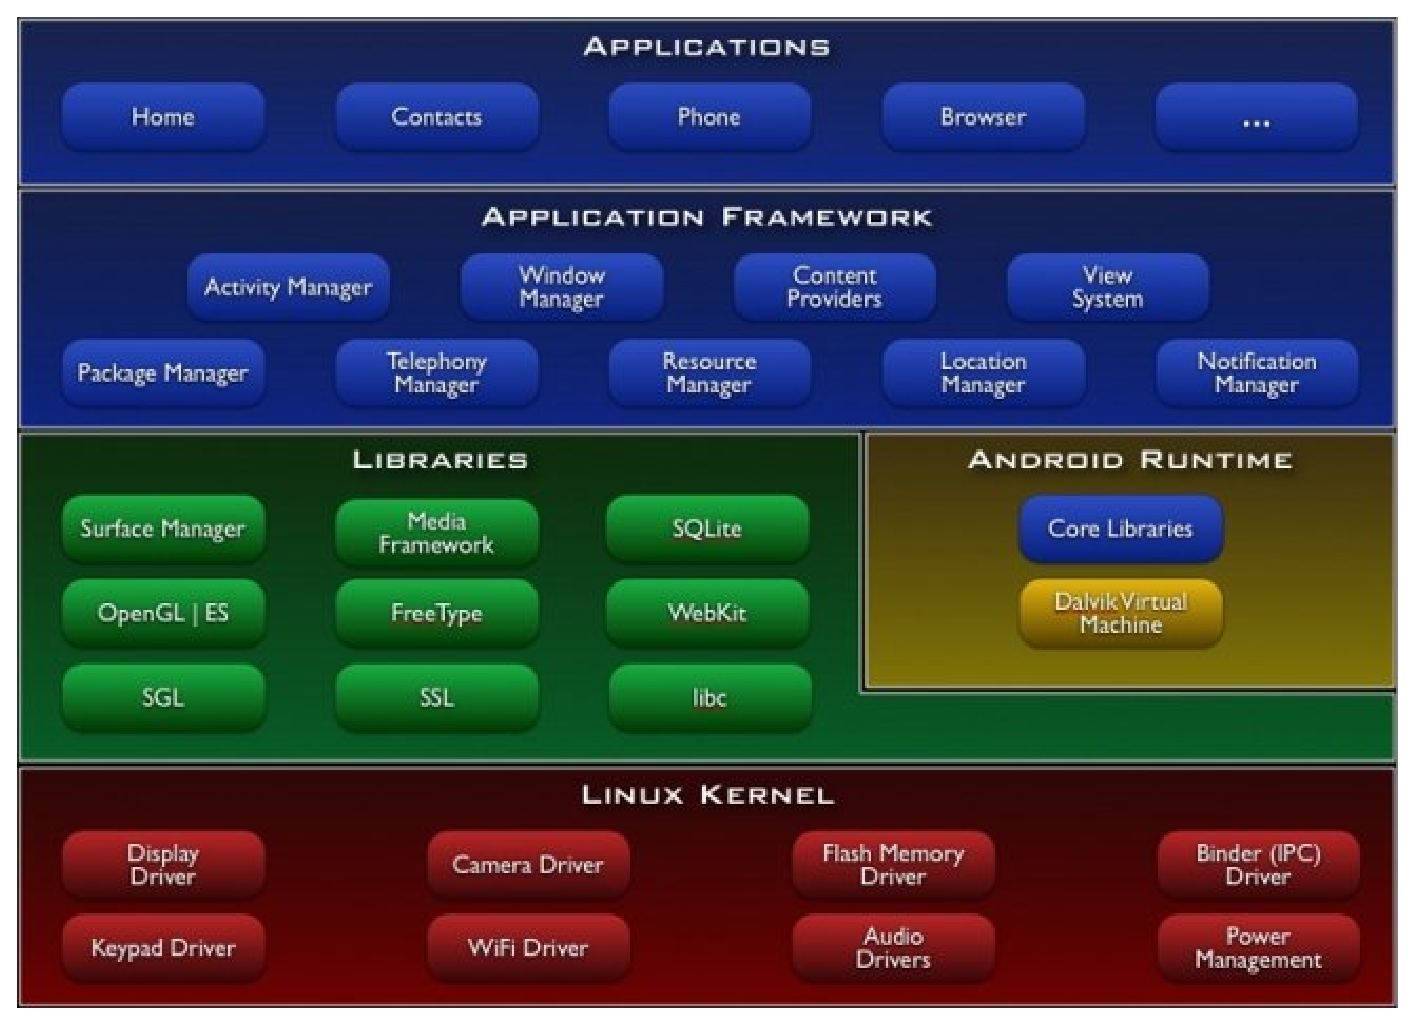
\includegraphics[width=0.9\textwidth]
{imagini/arhitectura-sistem.eps}
\end{center}
\end{figure}

\section{Linux Kernel}
\vspace{1cm}
Nivelul de bază al platformei Android este Linux kernel, acesta utilizându-se de binecunoscutul Linux kernel pentru a furniza funcționalitatea sistemului de operare.\newline


 Pentru a satisface nevoile dispozitivelor mobile, nucleul Linux pe care se bazează Android a suferit schimbări arhitecturale. Cele mai notabile fiind cele ce vor fi prezentate în următoarea secțiune.\newline
\newpage
\textbf{Binder}\newline
Arhitectura platformei Android se folosește intens de comunicația între procese (inter-process communication-IPC). Aplicațiile comunică cu sistemul, telefonul, serviciile și între ele utilizând IPC. Având în vedere că mecanismul IPC furnizat de sistemul de operare Linux nu este suficient, platforma Android a dezvoltat propriul sistem IPC, cunoscut sub numele de Binder, acesta fiind canalul central de comunicație al întregii platforme Android.\newline 
Deoarece Binder este implementat ca un serviciu de bază in Linux kernel Android, dezvoltatorii de aplicații nu interacționează direct cu acesta. Majoritatea API-urilor \footnote{application programming interfaces } frameworkului Android se bazează pe Binder pentru a interacționa cu platforma într-un mod transparent dezvoltatorului de aplicații.\newline
 Pentru a utiliza Binder în interacționarea cu alte aplicații din sistem, SDK-ul Android \footnote{Android Software Development Kit } furnizează  Android Interface Definition Language (AIDL).  AIDL cuprinde funcționalitatea de a descompune obiectele primite în primitive astfel încât Binder le poate înțelege și utiliza dincolo de limitele procesului.\cite{2}\newline

\textbf{Logger}\newline
Logger este mecanismul esențial pentru depanare. Având în vedere faptul că aplicațiile mobile depind mult de elemente din mediul înconjurător cum ar fi rețelele WiFi și de datele care provin de la anumiți senzori ai dispozitivului, funcționalitățile de logare ale aplicației nu sunt îndeajuns de bune pentru probleme complexe. De aceea, este esențial să combinăm funcționalitățile de logare ale sistemului cu cele ale aplicației pentru o imagine complexă.\newline 
Acest lucru devine mai greu de obținut atunci când dezvoltarea aplicației și executarea acesteia au loc pe mașini diferite.\newline
Android furnizează un sistem larg de servicii de logare care agreghează logările care provin din partea platformei Android și cele care provin de la aplicațiile care rulează pe aceasta.\newline 
SDK-ul Android-ului furnizează de asemenea uneltele necesare pentru a monitoriza logările în timp real și suport pentru filtrare avansată.\cite{2}\newline

\textbf{Wake Locks}\newline
Platforma Android este dezvoltată pentru a opera pe dispozitive mobile cu resurse limitate. Puterea bateriei este cea mai importantă și de aceea, dispozitivele Android intră in modul low-powered, numit și sleep. Chiar dacă acest mod permite utilizarea rezervei de baterie rămasă într-un mod eficient, nu este indicat ca un dispozitiv să intre în modul sleep pe parcursul unei operațiuni importante ale unei aplicații sau a unui serviciu.\newline
 Wake locks au fost introduse în Linux kernel al platformei Android cu scopul de a preveni aplicațiile de la intrarea in modul sleep.\cite{2}\newline

\textbf{Alarm Timer\footnote{în română, cronometru}}\newline
La fel cum am menționat anterior în secțiunea ,,Wake Locks'', dispozitivele intră în modul sleep pentru a conserva puterea bateriei. Pe parcursul modului sleep, nicio aplicație Android nu poate rula. Din acest motiv, a fost introdus alarm timer-ul care permite aplicațiilor să programeze sarcinile de execuție. \cite{2}\newline

\textbf{Low Memory Killer}\newline
La fel ca și bateria, memoria este de asemenea o resursă limitată a dispozitivelor mobile. Pe lângă dimensiunea memoriei, încărcarea în memorie a aplicațiilor este de asemenea o operație costisitoare. Pentru a rezolva aceasta problemă, platforma Android menține toate aplicațiile deschise încărcate în memorie chiar dacă utilizatorul nu mai interacționează cu ele.\newline
 Acest lucru permite utilizatorului o interschimbare rapidă între aplicații.\newline
 Această optimizare vine însă cu un cost: dispozitivul poate rămâne repede fără memorie dacă mai multe aplicații sunt deschise. \newline
 Low Memory Killer cunoscut și ca Viking Killer, a fost introdus în Linux kernel al platformei Android pentru a administra și a revendica memoria înainte ca dispozitivul să rămână fără aceasta.\newline
 Atunci când memoria disponibilă scade sub un anumit prag, low memory killer, elimină din memorie aplicațiile pornite, începând cu cele mai puțin importante.\newline
 Importanța unei aplicații este definită după vizibilitatea acesteia pentru utilizator.\newline
 O aplicație care rulează în prim plan este considerată cea mai importantă iar o aplicație care rulează pe fundal nu este considerată importantă. Stările curente ale aplicațiilor închise sunt salvate și pot fi reluate când utilizatorul se întoarce la o aplicație.\cite{2}\newline


\textbf{File System}\newline
Platforma Android se bazează pe Yet Another Flash File System (YAFFS2) ca și tip primar de sistem de fișiere, fiind dezvoltat pentru a lucra pe NAND-based flash chips. Sistemul de fișiere Android este de asemenea structurat într-un mod specific pentru a fi posibilă o actualizare ușoară a unor porțiuni ale platformei, aceste modificări neavând impact asupra celorlalte părți. Acest lucru este realizat prin menținerea porțiunilor platformei Android în partiții de sistem diferite, astfel garantându-se și o securitate mai ridicată întrucât componentele cheie ale platformei nu sunt mutabile pe parcursul rulării, evitând infectarea cu viruși și malware a componentelor cheie ale sistemului de operare.\cite{2}\newpage

Partițiile utilizate depind de producătorii dispozitivelor, cele mai des întâlnite fiind următoarele:\newline
\begin{itemize}
  \item /boot
  \item /system
  \item /recovery
	\item /data
	\item /cache
\end{itemize}

\section{Native Libraries}
\vspace{1cm}
Pe nivelul superior nucleului Linux, platforma Android conține un set de biblioteci native, precum:
\begin{itemize}
\item SQLite: Furnizează o memorie internă ce relaționează cu o bază de date SQL pentru persistența datelor și accesarea rapidă a acestora într-un mod structurat
\item WebKit:  Furnizează suport de interpretare HTML/CSS  și un motor de executare JavaScript pentru a permite aplicațiilor Android să încorporeze tehnologii web
\item OpenGL ES: Furnizează funcționalități performante pentru grafica 2D si 3D
\item Open Core: Furnizează un framework media care permite aplicațiilor Android să înregistreze și să redea conținut audio și video
\item Open SSL: Furnizează protocoalele Secure Socket Layer (SSL)  și Transport Level Security (TLS) care permit aplicațiilor Android să comunice în mod securizat cu servicii la distanță prin utilizarea criptografiei
\end{itemize}\cite{1}

\section{Android Runtimes}
\vspace{1cm}
Android Runtime este porțiunea care dirijează platforma Android, rulând atât serviciile platformei cât și aplicațiile care rulează pe platformă.\newline

\textbf{Android Runtime (ART)}
\newline
Limbajul de programare oficial folosit pentru Android este Java. Java este un limbaj de programare obiect-orientat specific dezvoltării de aplicații independente de platforma de lucru.
Acest lucru este posibil deoarece codul Java compilat al aplicației este realizat într-un limbaj independent de platformă numit bytecode. Acest bytecode este executat de Java Virtual Machine care rulează pe platformă.\newline

The Android Runtime (ART) este noul Java Virtual Machine ce a fost introdus într-un mod experimental în versiunea de Android 4.4, ca mai apoi să fie introdus în versiunea Android 5.0 ca runtime-ul oficial al aplicațiilor Android.  Înainte de versiunea 5.0, aplicațiile Android rulau pe Dalvik Virtual Machine (VM).\newline
În comparație cu abordarea Dalvik VM’s just-in-time (JIT) , ART se bazează pe o abordare ahead-of-time (AOT) , care permite compilarea codului bytecode și translatarea lui în cod mașină pe timpul instalării aplicației. Acest lucru permite codului aplicației să fie executat în viitor direct din mediul de rulare al dispozitivului.\cite{1}\newline

\section{Android Applications}
\vspace{1cm}
\textbf{Compiled Android Applications}\newline
Chiar dacă oficial ART este runtime-ul utilizat pentru platforma Android începând cu versiunea 5.0, majoritatea dispozitivelor Android care rulează pe versiuni mai vechi de Android utilizează plaforma Dalvik VM. \newline
Pentru a produce pachete de aplicații care să fie compatibile atât cu ART cât și cu Dalvik VM, acestea sunt încă dezvoltate utilizând specificațiile Dalvik. \newline Deoarece a fost optimizat pentru dispozitive mobile, Dalvik VM procesează doar un tip special de bytecod numit Dalvik Executable (DEX). SDK-ul Androidului cuprinde unelte care pot traduce bytecode-ul standard din Java în bytecode DEX pe parcursul asamblării aplicației android. Utilizarea bytecode-ului DEX furnizează multe avantaje în comparație cu bytecode-ul standard Java. Art realizează conversia automată de la formatul Dalvik DEX la formatul ART OAT imediat după instalarea aplicației pe dispozitiv.\cite{1}\newline


\textbf{Application Sandbox}\newline
Platforma Android este construită având în vedere securitatea ca o necesitate importantă. Astfel rulează fiecare aplicație într-un sandbox izolând datele aplicației și codul executabil de alte aplicații.\newline
- Fiecare aplicație rulează pe instanța ART VM dedicată. \newline
- Datele aplicației sunt protejate prin utilizarea unui fișier cu permisiuni ale sistemului. Fiecare aplicație are asignat un cont la instalare și sistemul de operare restricționează accesul la date pentru acel cont.\newline
- Aplicațiile pot să comunice cu sistemul sau cu alte aplicații prin interfața de comunicare pe care platforma Android o pune la dispoziție. Aceste interfețe sunt de asemenea protejate prin permisiuni Android\cite{1}.\newline

\textbf{Application Framework}\newline
Framework-ul aplicației rulează pe ART VM și dispune de o interfață pentru ca aplicațiile Android să interacționeze cu platforma Android și cu dispozitivul mobil. Cuprinde servicii precum : Package Manager, Telephony Manager, Location Manager, and Notifications Manager.\cite{1}\newline


\textbf{Applications}\newline
Spațiul aplicațiilor cuprinde toate aplicațiile Android cu care se confruntă utilizatorul care rulează pe ART VM. Aceste aplicații includ și aplicațiile de la terți, care sunt downloadate din magazinul Android și aplicațiile de sistem precum Aplicația de pornire(Launcher), Contacte(Contacts), Telefon(Phone) și Browser. \cite{1}\newline

\section{Versiuni Android}
\vspace{1cm}
\begin{center}
\begin{figure}[htbp]
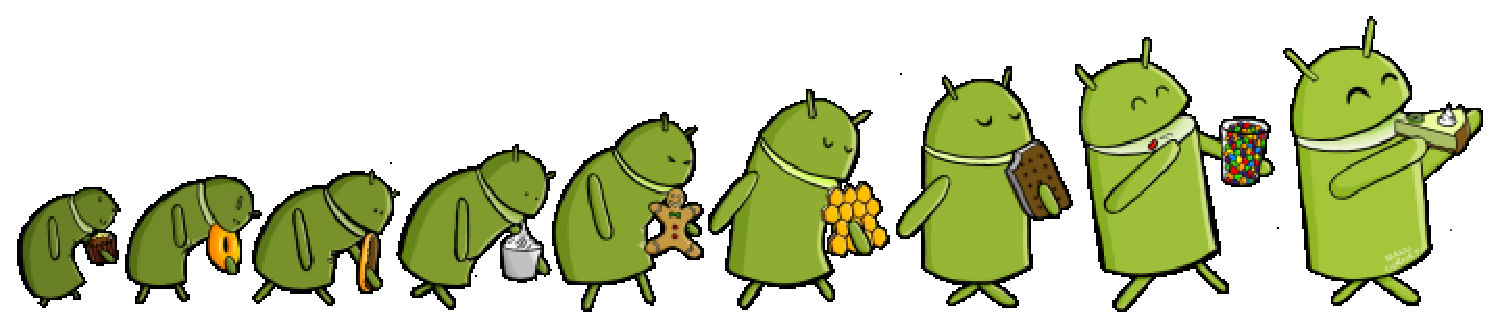
\includegraphics[width=0.9\textwidth]
{imagini/androidVersions.eps}
\end{figure}
\end{center}
Dezvoltarea sistemul de operare Android a început în 2003 de Android Inc. care a fost apoi cumpărat de Google in 2005.[3]
Cea mai recentă actualizare a sistemului Android este versiunea Android 5.0 ,,Lollipop'', care a fost lansată în 3 Noiembrie 2014. Începând cu Aprilie 2009, versiunile Android au fost denumite cu nume de deserturi, fiind lansate în ordine alfabetică, începand cu Android 1.5 ``Cupcake'', versiunile anterioare 1.0 Alpha si 1.1 Beta fiind versiuni pre-comerciale.\cite{9}\newline
\begin{center}
\begin{table}\includegraphics[width=0.9\textwidth, height=0.8\textheight]
\begin{tabular}{|p{5cm}|p{1.5cm}|p{3cm}|p{1.5cm}|}\hiderowcolors
\hline
\cellcolor{LightPink} Data lansării & \cellcolor{LightGreen} Versiune & \cellcolor{LightPink} Nume  & \cellcolor{LightGreen} Nivel API \\
September 2008& 1.0& -- & 1\\
\hline
February 2009& 1.1& -- & 2\\
\hline
April 2009& 1.5& Cupcake& 3\\
\hline
September 2009&1.6& Donut& 4\\
\hline
October 2009& 2.0& Éclair& 5\\
\hline
December 2009& 2.0.1& Éclair& 6\\
\hline
January 2010& 2.1& Éclair& 7\\
\hline
May 2010& 2.2–2.2.3& Froyo& 8\\
\hline
December 2010& 2.3–2.3.2& Gingerbread& 9\\
\hline
February 2011& 2.3.3–2.3.7& Gingerbread& 10\\
\hline
February 2011& 3.0& Honeycomb& 11\\
\hline
May 2011& 3.1& Honeycomb&12\\
\hline
July 2011& 3.2–3.2.6& Honeycomb& 13\\
\hline
October 2011& 4.0–4.0.2& Ice Cream Sandwich& 14\\
\hline
December 2011& 4.0.3–4.0.4& Ice Cream Sandwich& 15\\
\hline
July 2012& 4.1–4.1.2& Jelly Bean& 16\\
\hline
November 2012& 4.2–4.2.2& Jelly Bean& 17\\
\hline
July 2013& 4.3–4.3.1& Jelly Bean& 18\\
\hline
October 2013& 4.4–4.4.4& KitKat& 19\\
\hline
July 2014& 4.4w& KitKat with Wearable Extensions& 20\\
\hline
November 2014& 5.0& Lollipop& 21\\
\hline
\end{tabular}
\caption{Versiuni Android}
\end{table}
\end{center}
În 3 septembrie 2013, Google anuntă că un miliard de dispozitive Android activate sunt folosite în toată lumea. \newline 
În Ianuarie 2015, Android deține 62\% din piața de smartphone-uri și tablete din US, 82.7\% din piața chineză și 73.3\% din piața europeană. \cite{9} \newpage

\section{Android Platform Fragmentation}
La o simplă vedere a datelor de lansare prezentate in tabelul 1-1, este posibil sa credeți că cele mai multe dispozitive Android ruleaza pe minim versiunea Android 4.4, însă acest lucru nu este adevărat. \newline 
Datorită fragmentării mari, datele de lansare nu oferă o imagine clară a ecosistemului Android.\newline 
Tabelul 1 este cel mai recent grafic de distribuție a versiunilor de Android Dashboard2 \cite{2} pe baza datelor colectate în luna decembrie 2014.\cite{1}\newline 


\begin{table}[!hp]
\caption{Distribuția versiunilor Android}
\begin{tabular}{|c|c|c|c|}
\hline
\cellcolor{LightPink}Versiune & \cellcolor{LightGreen} Nume versiune & \cellcolor{LightPink} Nivel API &\cellcolor{LightGreen} Nivel distribuție\\
\hline
2.2–2.2.3& Froyo& 8& 0.5\%\\
\hline
2.3.3–2.3.7& Gingerbread& 9& 9.1\%\\
\hline
4.0.3–4.0.4& Ice Cream Sandwich& 15& 7.8\%\\
\hline
4.1–4.1.2& Jelly Bean& 16& 21.3\%\\
\hline
4.2–4.2.2& Jelly Bean& 17& 20.4\%\\
\hline
4.3–4.3.1& Jelly Bean& 18& 7.0\%\\
\hline
4.4–4.4.4& KitKat& 19& 33.9\%\\
\hline
\end{tabular}
\end{table}


După cum se observă în tabelul 1-2, versiunea de Android 4.4 cuprinde doar sistemele de operare ale 33.9\% de utilizatori din numărul total al acestora. Dezvoltarea unei aplicații Android având ca target doar nivelul API 19 va limita audiența la numai 33.9\% dintre utilizatorii de bază Android.
\newline Cu toate că un nivel API superior furnizeaza funcționalităti suplimentare, este de preferat sa luăm în calcul diagrama de distribuție pentru a determina numărul audienței.\cite{1}

\section{Android Support Library}
Chiar dacă setarea unui target API mai mic mărește numărul de persoane care vor putea utiliza aplicația, de asemenea limitează funcționalitățile de care putem să ne folosim în dezvoltarea unei aplicații Android. Pentru a remedia această problemă, a fost introdus Android Support Library.
Acest pachet pune la dispoziție versiuni anterioare compatibile ale API-urilor recente.\newline 
Acest lucru inseamnă că o aplicație care este dezvoltata pentru nivelul API 19 poate avea ca target nivelele API 4 și nivelurile următoare.\newline 
Includerea bibliotecii Android Support Library într-o aplicație este considerată o tehnică ,,best practice''.\cite{1}

\chapter{Componetele unei aplica\c tii Android}

Framework-ul Android ofer\u a o serie de componente pentru dezvoltarea de aplica\c tii consistente \c si interoperabile. \^In continuare vor fi prezentate componentele fundamentale oferite de platforma Android.\cite{3}
\begin{center}
\begin{figure}[!hp]
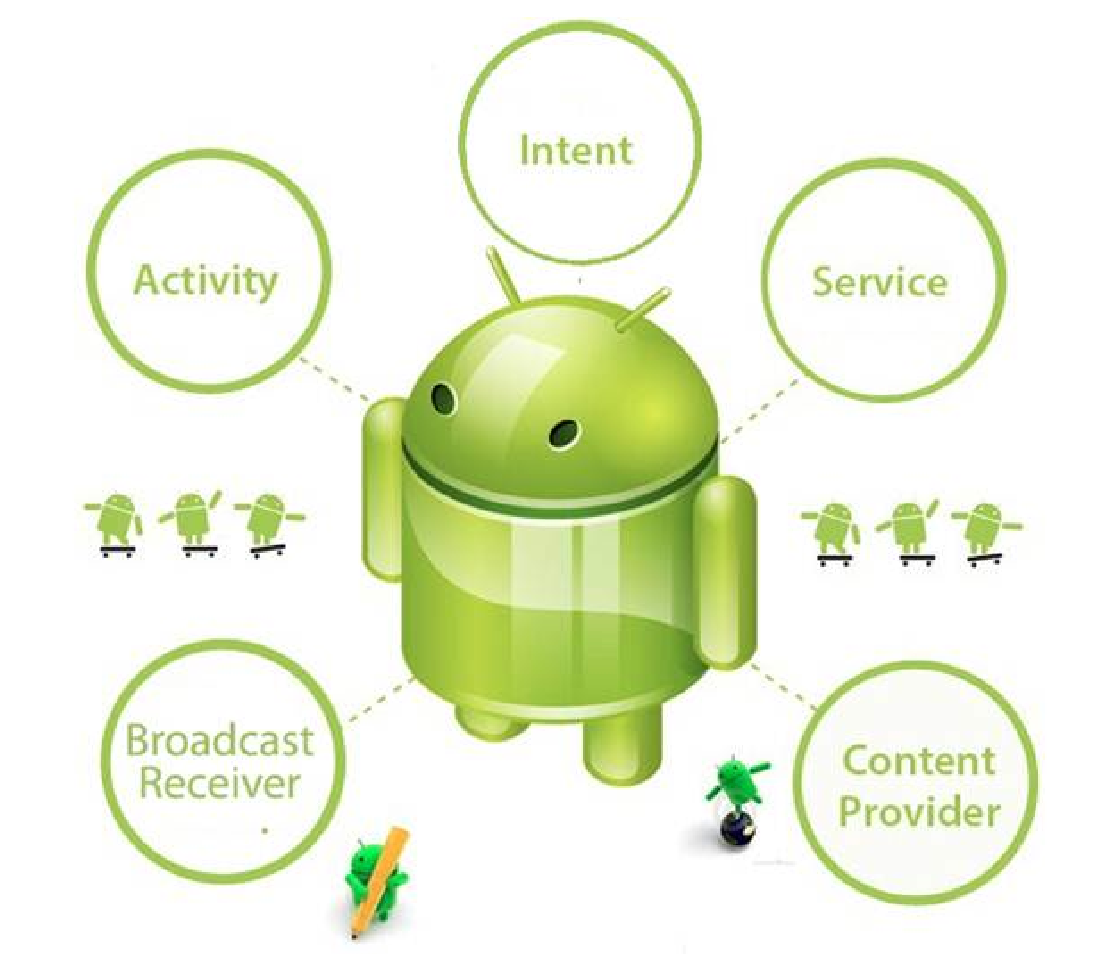
\includegraphics[width=0.65\textwidth]
{imagini/components-of-android.eps}
\end{figure}
\end{center}

\section{Activity}

,,Activity'' este numele dat pentru o aplica\c tie \^in care utilizatorul poate interac\c tiona cu o singur\u a fereastr\u a la un moment dat. A fost ales numele de ,,activitate'' pentru a sugera faptul c\u a aplica\c tia poate s\u a realizeze o singur\u a func\c tionalitate focusat\u a pe utilizator.\newline 
Pe platforma Android, acest aspect de limitare al domeniului fiecarui ecran aduce func\c tionalitea de interac\c tionare cu alte aplica\c tii. De exemplu, la utilizarea e-mail-ului pe un dispozitiv mobil, c\^and userul are posibilitatea de a selecta un contact din lista de contacte c\u aruia s\u a-i trimit\u a e-mail-ul.\newline 

Acest lucru face posibil\u a reutilizarea codului \c si men\c tinerea platformei in str\^ans\u a leg\u atura.\newline
Aproape toate aplica\c tiile necesit\u a comunicarea \c si/sau interac\c tionarea cu un client, \c si din acest motiv, activitatea se ocup\u a de crearea unei ferestre \c si de a\c sezarea componentelor interfetei utilizator.\cite{3}\newline 

\subsection{Crearea unei activit\u a\c ti}
Pentru a crea o nou\u a activitate se deriveaz\u a o clasa din android.app.Activity, dup\u a cum putem observa \^in exemplul 3.1.\cite{3}\newline 

\begin{exmp} Crearea unei activit\u a\c ti\newline 
import android.app.Activity;\newline 
public class MyActivity extends Activity \{\newline 
\}\end{exmp}

\subsection{Declararea unei activit\u a\c ti}
Derivarea unei clase de acvitate nu \^inseamn\u a \c si faptul c\u a acea activitate este automat utilizabil\u a. Pentru ca o activitate s\u a ia anumite roluri \^in aplicatie, platforma Android necesit\u a ni\c ste meta-informa\c tii despre noua activitate. Aceste informa\c tii sunt furnizate de c\u atre fisierul XML Android manifest, unde eticheta XML /<activity/> declar\u a noua activitate prin precizarea numelui de clas\u a, a titlului \c si a modului \^in care va fi expus\u a utilizatorului.\cite{1}\newpage

\subsection{Ciclul de via\c t\u a al unei activit\u a\c ti}\cite{1}

\begin{center}
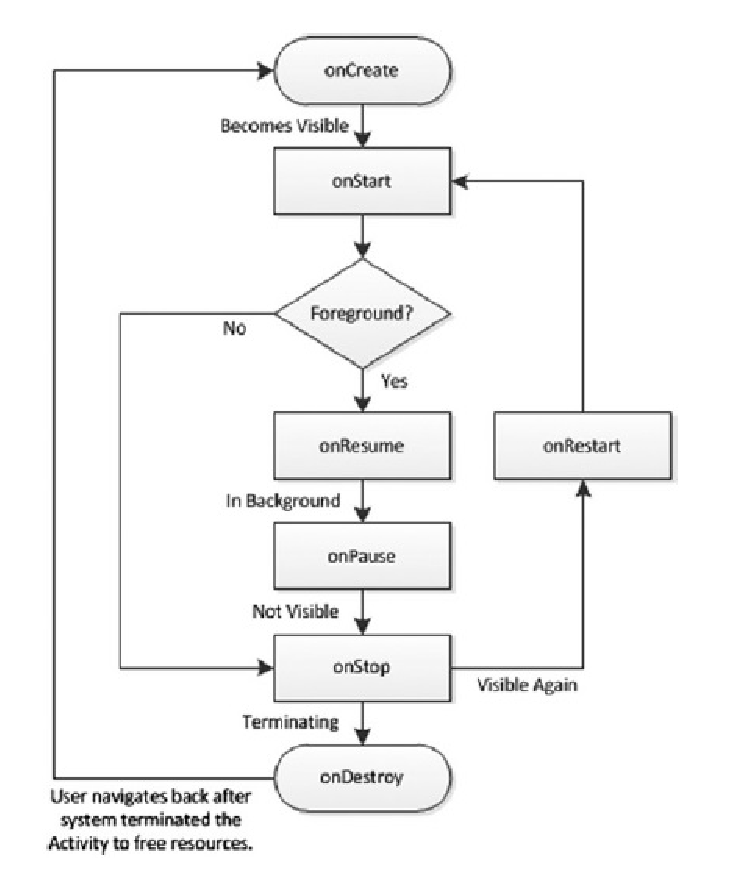
\includegraphics[width=0.6\textwidth]{imagini/activity.eps}
\end{center}

\section{Intent}
Dup\u a cum am men\c tionat \c si anterior, platforma Android este dezvoltat\u a pentru a fi extrem de modular\u a, promov\^ and colaborarea dintre aplica\c tiile prezente pe dispozitiv. Astfel, aplica\c tiile pot \^imbina activit\u a\c ti pentru a oferi o anumit\u a func\u tionalitate utilizatorului. Acest lucru este posibil printr-un binding runtime \^int\^arziat, cunoscut sub numele de android.content.Intent, pe care platforma Android \^il pune la dispozi\c tie.\newline 
Intent-ul de\c tine o structur\u a pasiv\u a de date care memoreaz\u a o descriere abstract\u a a ac\c tiunii ce urmeaz\u a a fi \^intreprins\u a. Principalele informa\c tii dintr-un intent sunt:\newline 

\begin{itemize}
  \item action, care reprezint\u a \^in general ac\c tiunea ce va fi \^intreprins\u a
  \item data, care reprezint\u a un obiect URI (uniform resource identifier) ce se refer\u a la datele care vor fi prelucrate
\end{itemize}
Cea mai important\u a utilizare a intentului este de a lansa activit\u a\c tile si serviciile.

\section{Service}
Pentru aplica\c tii cu durat\u a de rulare mai mare, durata de via\c t\u a a unei activit\u a\c ti s-ar putea s\u a nu fie indeajuns de lung\u a, de exemplu daca o aplica\c tie necesit\u a desc\u arcarea de pe Internet a unui videoclip, platforma va termina activitatea imediat dup\u a ce utilizatorul p\u araseste temporar aplica\c tia fără a verifica dac\u a opera\c tia s-a incheiat sau nu.\newline 
Framework-ul Android furnizeaz\u a o component\u a a aplica\c tiei, numit\u a android.app.Service, pentru a permite aplica\c tiilor s\u a execute opera\c tii cu durrata de rulare mai mare \^in planul secundar.\newline 
Serviciile pot fi utilizate \c si din aceeasi aplica\c tie dar \c si de alte aplica\c tii  de pe dispozitiv dac\u a serviciul este exportat.\cite{1}


\subsection{Crearea unui Service}
Crearea unui serviciu se face prin simpla derivare a unei noi clase din android.app.Service cum se vede \^in exemplul 3.2.\cite{2}\newline 
\begin{exmp} Crearea unui Service
import android.app.Service;\newline 
public class MyService extends Service \{ \newline 
\} \end{exmp}

\subsection{Declararea unui Service}
Crearea unui noi serviciu nu \^il face imediat utilizabil pe platforma Android. Aceasta are nevoie de meta-informa\c tii pentru a putea utiliza serviciul. Aceste meta-informa\c tii se g\u asesc \^, de asemnea \^in  fi\c sierul Android manifest fiind marcate cu tagul XML <service>.\newline 
Asemenea elementului <activity>, elementul <service> poate s\u a con\c tina elemente <intent-filter> \^in corpul s\u au pentru a specifica ce ac\c tiuni s\u a indeplineasc\u a.\cite{2}

\subsection{Ciclul de via\c t\u a al unui Service}
\begin{center}
\caption{\cite[1]}
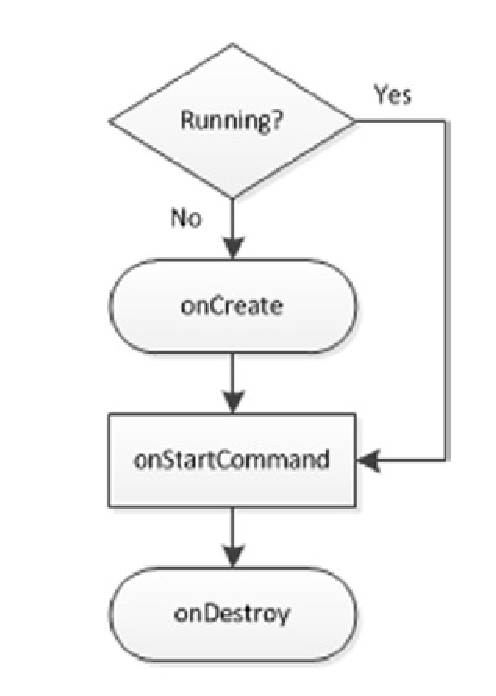
\includegraphics[width=0.3\textwidth]{imagini/service.eps}
\end{center}

\newpage
\section{Content Provider}
Dup\u a cum am men\c tionat anterior \^in sec\c tiunea ,,Service'', at\^ at activit\u a\c tile c\^ at \c si serviciile pot fi exportate astfel \^incat alte aplicatii care ruleaz\u a pe acela\c si dispozitiv mobil s\u a poat\u a interac\c tiona simultan cu acestea. Chiar dac\u a accesarea unor p\u ar\c ti ale altor aplica\c tii poate fi foarte util\u a, \^in anumite cazuri, este nevoie de simpla accesare a datelor, f\u ar\u a accesarea anterioar\u a a activit\u a\c tilor si a serviciului.\newline 
Platforma Android furnizeaza o component\u a aplica\c tiei, numit\u a content provider, care manageriaz\u a accesul la un set structurat de date. Este o interfa\c t\u a standard care conecteaz\u a datele unei aplica\c tii cu codul executabil al altei aplica\c tii.\cite{2}\newline 

\subsection{Crearea unui Content Provider}
Un nou content provider poate fi creat prin simpla derivare a unei noi clase din android.content.ContentProvider ca \^in exemplul 3.3.\newline 
\begin{exmp} Crearea unui Content Provider 
import android.content.ContentProvider;\newline 
public class MyContentProvider extends ContentProvider \{\newline 
\}\end{exmp}

Clasa abstract\u a ContentProvider cuprinde 6 metode abstracte care necesită implementare.\cite{2}

\begin{itemize}
  \item query - metodă apelat\u a pentru a interoga providerul pentru date 
  \item insert - metodă apelat\u a pentru a insera continut nou in provider
	\item update - metodă apelat\u a pentru a actualiza continutul unui provider cu un nou conținut
	\item delete-  metodă  apelat\u a pentru a sterge providerul
	\item getType -metodă apelat\u a pentru a prelua tipul MIME pentru conținutul ce va fi returnat pentru URI-ul dat
	\item onCreate - metodă apelat\u a de platform\u a c\^and se instan\c tiaz\u a providerul.(apelat\u a inainte de orice altă metod\u a)
\end{itemize}
\newpage
\section{Broadcast Messages}
Platforma Android furnizeaz\u a un sistem larg de mesagerie numit broadcast messages. Aceast\u a facilitate permite aplica\c tiilor \c si sistemului s\u a propage evenimente \c si schimb\u ari de stare pentru par\c tile interesate prin emiterea unui intent ca mesaj.\newline 
Un mesaj broadcast poate fi trimis prin metoda sendBroadcast. \newline 
Pentru receptarea unui mesaj broadcast, aplica\c tia trebuie s\u a deriveze o nou\u a clas\u a din android.content.BroadcastReceiver. \newline 

Simpla derivare a clasei nu este ins\u a suficientă pentru a recep\c tiona mesajele. Aplica\c tia trebuie s\u a informeze platforma Android dinamic prin cod sau prin \^inregistrarea \^in fisierul manifest cu privire la intenția de a recep\c tiona mesaje broadcast.\newline
Tagul XML <receiver> este utilizat pentru a \^inregistra un receptor broadcast \^in manifestul aplica\c tiei.\newline
Pentru \^inregistrarea dinamic\u a prin cod, exist\u a metoda registerReceiver.\cite{1}\newline

\chapter{Limbajul de programare Java}

\section{Platforma Java}
\vspace{1cm}
\begin{defn}
Java este un limbaj de programare orientat-obiect, puternic tipizat, conceput de către James Gosling la Sun Microsystems (acum filială Oracle) la începutul anilor '90, fiind lansat în 1995. Cele mai multe aplicații distribuite sunt scrise în Java, iar noile evoluții tehnologice permit utilizarea sa și pe dispozitive mobile gen telefon, agenda electronică, palmtop etc. În felul acesta se creează o platformă unică, la nivelul programatorului, deasupra unui mediu eterogen extrem de diversificat. Acesta este utilizat în prezent cu succes și pentru programarea aplicațiilor destinate intranet-urilor. \cite{12}
\end{defn}
Java este un limbaj de programare utilizat în toate industriile pentru aproape orice tip de aplicație. Există aproximativ 6 milioane de programatori Java în lume, însă sunt de asemenea și multe posturi disponibile, astfel că un programator care are cunoștințe medii de programare Java are mai multe șanse să-si gasească un job față de un programator expert în alte limbare de programare precum C/C++, Ruby, etc.
\paragraph{ }Java a apărut pe scena tehnologiei în anul 1995 și a devenit popular foarte repede. Acest lucru s-a întâmplat în parte din cauza JVM.
JVM este ca un translator de limbi străine, având loc transformarea bytecode-ului Java în orice limbaj nativ ce poate fi interpretat de un anumit calculator.\cite{10}\newline
Programele Java sunt rulate (sau interpretate) de către un alt program numit Java VM. Programele nu rulează direct pe sistemul de operare nativ, ci sunt interpretate de Java VM pentru sistemul de operare nativ.\newpage Acest lucru înseamnă că orice sistem de operare cu Java VM instalat poate rula programe Java, indiferent de sistemul de operare pe care au fost dezvoltate inițial aplicațiile.\newline
 Aceasta se numește portabilitate, și în lumea programării, portabilitatea este un produs foarte prețios.\cite{11} \newline

Platforma Java constă în API-ul Java și mașina virtuală Java (JVM).

\paragraph{ }API-urile Java sunt biblioteci de cod compilat care se folosesc în dezvoltarea programelor java. Acestea permit adăugarea unor funcționalității personalizabile pentru a economisi timp de programare, unul dintre cele mai simple exemple fiind reprezentat de API-ul folosit pentru a printa o linie de cod în consolă; comanda pentru printare în consolă este furnizată din API și poate fi folosită numai prin specificarea textului ce va fi printat. \newline

De exemplu, un program Java dezvoltat pe un computer personal (PC) cu sistemul de operare Windows NT ar trebui să ruleze la fel de bine fără modificări pe o stație de lucru cu sistem de operare Linux, și vice-versa.\cite{10}\newline 

\section{Configurarea unui computer}

Pentru a scrie programe Java, sunt necesare:
\begin{itemize}
  \item un compilator Java
	\item un JVM
	\item API-ul Java
	\item acces la documentația API-ului Java
	\item un editor pentru redactarea programelor Java.
	\item un program care să interpreteze și să execute comenzile redactate 
\end{itemize}
Pentru ultimele două acțiuni se folosește, în general, o singură interfață prietenoasă, numită mediu de dezvoltare integrat(integrated development environment - IDE).
Printre cele mai cunoscute IDE - uri utilizate pentru dezvoltarea de aplicații Java se numără: Eclipse, NetBeans, IntelliJ IDEA, JDeveloper, JCreator, etc.\newpage

În procesul de realizare a aplicației mele, am utilizat pentru programul de citire a link-urilor și actualizarea periodică a bazei de date,  ca și mediu de dezvoltare integrat Eclipse IDE, deoarece:\newline
\begin{itemize}
	\item poate fi descărcat și apoi utilizat gratuit
	\item este în topul celor mai utilizate Java IDE-uri de către programatorii consacrați
	\item este intuitiv și ușor de utilizat
\end{itemize}
\paragraph{ }Eclipse nu este folosit doar pentru dezvoltarea unei aplicații Java, ci poate fi folosit împreună cu o serie de alte limbaje de programare (Ada, ABAP, C, C++, COBOL, Fortran, Haskell, JavaScript, Lasso, Lua, Natural, Perl, PHP, Prolog, Python, R, Ruby, Scala, Clojure, Groovy, Scheme și Erlang), acest lucru reprezentând un plus semnificativ al acestui IDE.\newline



\textbf{JDK și JRE}\newline
Pentru dezvoltarea de programe Java pe un computer este nevoie să fie instalat JDK. Pentru rularea de programe Java care au fost compilate deja pe un alt computer, este de ajuns Java Runtime Environment (JRE). 
JDK include si JRE.

\section{Limbaj de programare obiect orientat}

Java este un limbaj de programare obiect orientat, ceea ce înseamnă că se pot construi si reprezenta obiecte din lumea reală. Fiecare program Java are cel putin o clasă care are anumite funcționalități. De exemplu, cea mai simplă clasă, HelloWorld, are funcționalitatea de a saluta lumea.
Clasele în Java pot să conțină metode(funcții) și atribute (proprietăți).\newline
\textbf{Principiile programării obiect orientate }\newline
\subsection{Abstractizarea datelor}
Abstractizarea datelor reprezintă procesul de definire a unui tip de date denumit tip abstract de date(abstract data type-ADT), recurgând și la ascunderea datelor.
Definirea unui tip abstract de date implică specificarea reprezentării interne a datelor pentru acel tip, precum și un set suficient de funcții cu ajutorul cărora putem utiliza acel tip fără a fi necesară cunoașterea structurii sale interne. \cite{15}

\subsection{Încapsularea}
Încapsularea se referă la ascunderea datelor și a metodelor într-un obiect., prin specificarea acestora ca fiind private în definiția clasei. Astfel, accesul la date se face doar prin intermediul metodelor descrise în clasă. Încapsularea este importantă pentru a asigura securitatea și integritatea obiectelor unei clase.  
Un mare avantaj al încapsulării este ascunderea implementării clasei astfel că metodele interne ale clasei pot fi modificate după cum vrea programatorul și atâta timp cât funcționalitatea externă nu este modificată, utilizatorul clasei nu va observa nicio diferență la utilizarea metodei.\cite{14}

\subsection{Moștenirea}
În limbajele de programare obiect-orientate, termenul de moștenire se referă la abilitatea de a defini o nouă clasă bazată pe una care deja există.
Clasa utilizată ca și clasă de bază poate fi definită de aceeași persoană, poate fi preluată de la altcineva sau dintr-un pachet Java specific.
Clasa derivată din clasa de bază se mai numește subclasă, clasă copil iar cea de bază se mai numește și superclasă, clasă părinte. 
Clasa derivată va moșteni de la superclasa sa toate funcționalitățile pe care aceasta le are dar poate să conțină și funcționalități noi sau să le suprascrie pe cele existente.\cite{14}

În figura următoare se observă o ierarhie de clase realizată prin moștenire:
\begin{figure}[!hp]
\centering
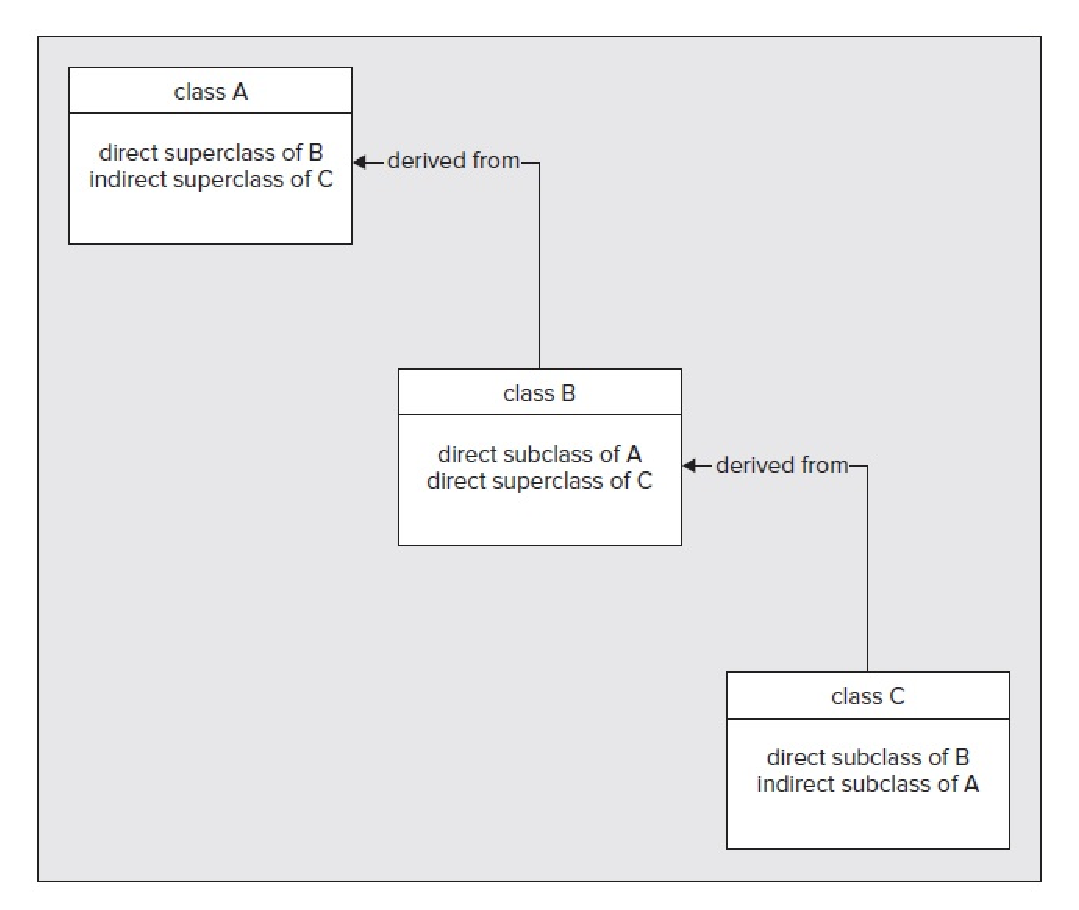
\includegraphics[width=0.9\textwidth]
{imagini/mostenire1.eps}
\end{figure}

După cum puteți vedea în Figura , o subclasă care se află în același pachet ca și clasa de bază moștenește totul cu excepția membrilor privați ai clasei de bază. Dacă se definește o subclasă în afara pachetului ce conține clasa de bază, atributele private nu sunt mostenite și nici ceilalți membrii din clasa de bază care au fost declarați fără specificator de acces sau cei declarați ca private.\newline
\begin{figure}[!hp]
\centering
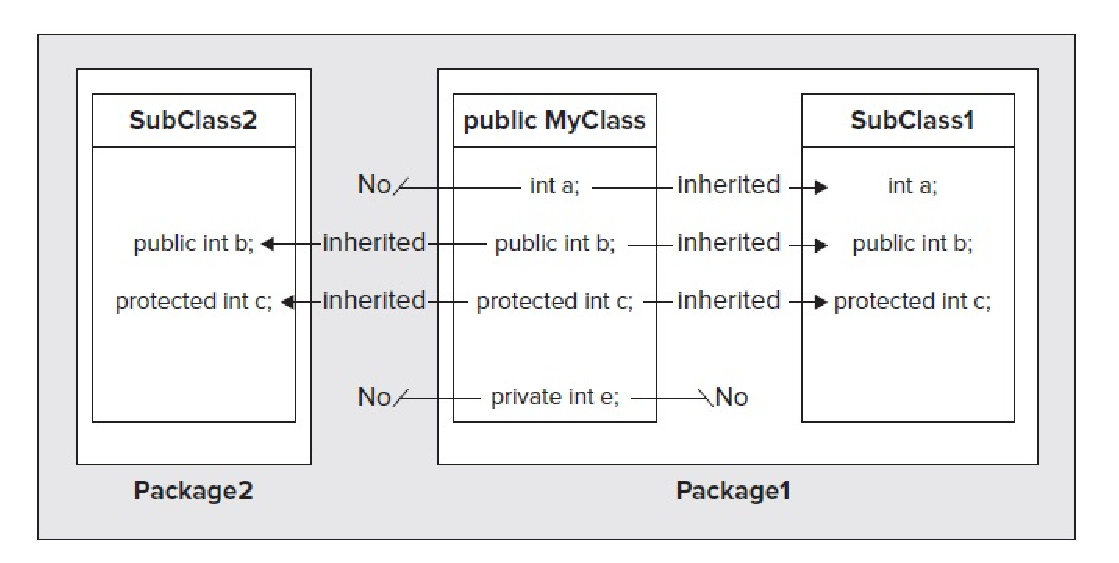
\includegraphics[width=0.9\textwidth]
{imagini/mostenire2.eps}
\end{figure}
Astfel, specificatorul public este cel mai puțin restrictiv, fiind vizibil oriunde, protected este următorul care previne accesul din clasele aflate în afara pachetului dar nu limitează moștenirea, clasa derivată poate să accese membrii clasei de bază declarați protected. Cel mai restrictiv specificator este private, accesul fiind valabil doar în interiorul clasei în care a fost declarat mebrul privat.

\subsection{Suprascrierea unei metode}
Un alt termen important din programarea obiect-orientată este reprezentat de către suprascrierea metodelor.
Putem defini o metodă într-o clasă derivată, care are aceeași semnătură ca și o metodă în clasa de bază. Având aceeași semnătură înseamnă că numele metodei trebuie să fie același și listele de parametri trebuie să conțină același număr de parametri cu tipuri identice. Atributul de acces pentru metoda în clasa derivată poate fi același cu cel din clasa de bază sau poate fi mai puțin restrictiv, dar nu poate fi mai restrictiv. Acest lucru înseamnă că, dacă declaram o metodă publică în clasa de baza, orice proprietate definită în clasa derivată trebuie să fie, de asemenea, declarată ca publică. Nu se poate omite atributul de acces în clasa derivată în acest caz, sau specificarea aceastuia ca fiind private sau protected.
Când se definește o nouă versiune a unei metode din clasa de bază în acest fel, metoda din clasă derivată suprascrie metoda din clasa de baz. \cite{14} \newline

\subsection{Adnotarea @Overriding}
Când se definește o metodă într-o clasă derivată, care este destinată pentru a suprascrie o metodă din superclasă, este ușor să se facă o greșeală în semnătura pentru metoda de clasă derivată. Dacă numele și lista de parametri din metoda clasei derivate nu sunt identice cu cele ale metodei din superclasa, are loc supraîncărcarea metodei din clasa de bază și nu suprascrierea acesteia. Pentru evitarea acestui lucru și pentru o mai bună lizibilitate a codului scris se folosește adnotarea @Overriding înainte de metoda care va suprascrie metoda din clasa de bază. Astfel compilatorul este informat și în caz că nu sunt indeplinite toate condițiile de suprascriere se va semnala o eroare de compilare.\cite{14} \newline

\subsection{Polimorfismul}
Polimosfismul înseamnă, în general, abilitatea de a avea mai multe forme. În programare, reprezintă abilitatea unei singure variabile de un tip dat să fie utilizată pentru a referi obiecte de tipuri diferite și să apeleze automat metoda specifică tipului obiectului referit. Aceasta presupune faptul că o singură metodă poate să se comporte diferit, în funcție de obiectul apelat.\newline
Acest lucru este evidențiat în figura următoare:\cite{14} 
\begin{figure}[!hp]
\centering
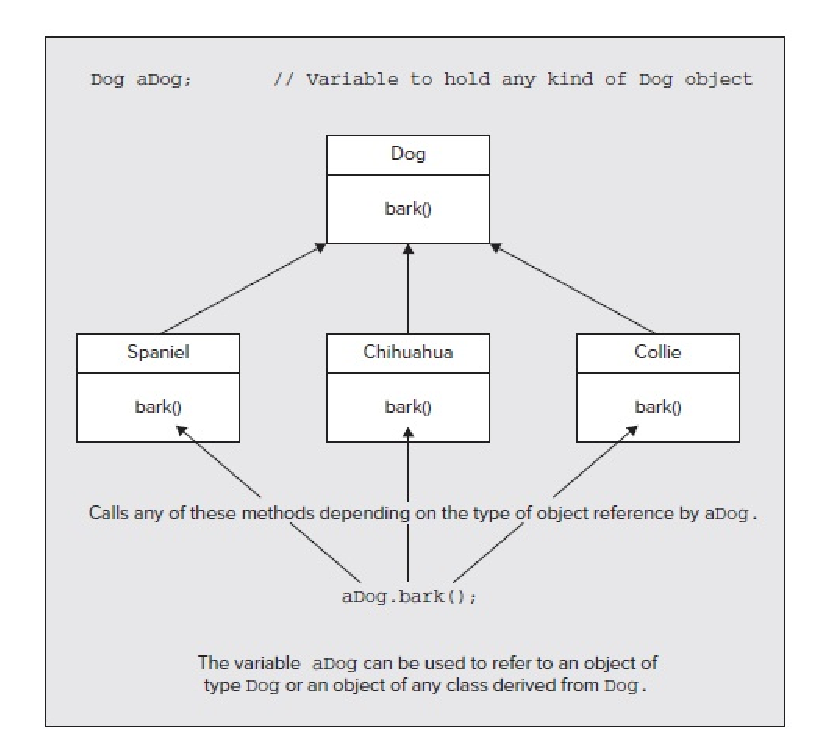
\includegraphics[width=0.9\textwidth]
{imagini/polimorfism.eps}
\end{figure}
\paragraph{}Condițiile care trebuiesc îndeplinite pentru a utiliza polimorfismul sunt următoarele:\cite{14} 
\begin{itemize}
	\item apelul metodei din clasa derivată trebuie să se facă prin intermediul unei variabile de tipul clasei de bază
	\item metoda apelată trebuie să fie definită în clasa de derivată
	\item metoda apelată trebuie să fie, de asemenea, declarată ca membru al clasei de bază
	\item semnătura metodei din clasa de bază trebuie să fie la fel cu semnătura metodei din clasa derivată sau tipurile returnate să fie covariante
	\item specificatorul de acces din clasa derivată nu trebuie să fie mai restrictiv ca specificatorul de acces din clasa de bază
\end{itemize}
\subsection{Clasa de bază universală}
Toate clasele definite în Java sunt implicit subclase ale clasei Object, nefiind nevoie să fie specificat acest lucru.
Astfel, cu ajutorul clasei Object, putem să scriem metode care vor utiliza obiecte de tipuri necunoscute, putem să definim parametri de tip Object, în acest fel metoda va putea fi folosită pentru orice tip de obiect trimis ca parametru. De asemenea, clasa Object cuprinde 7 metode publice și 2 protejate, pe care le vom vedea în tabelul următor:\cite{14} \newpage
\begin{center}
\begin{table}[!hp]
\caption{Metodele publice ale clasei Object}
\begin{tabular}{|p{4cm}|p{8cm}|}\hiderowcolors
\hline
\cellcolor{LightPink} Metodă & \cellcolor{LightGreen} Scopul metodei \\
toString()& Această metodă returnează un obiect String care descrie obiectul curent. În versiunea moștenită a acestei metode va fi returnat numele clasei urmat de ‘@’ și de reprezentarea hexazecimală a obiectului. Această metodă este apelată automat atunci când se concatenează obiecte cu variabile String utilizând operatorul +. Această metodă poate fi suprascrisă într-o clasă, pentru a crea un string personalizat pentru obiectul clasei. \\
\hline
equals() & Această metodă compară referința la obiectul trimis ca argument cu referința la obiectul curent și returnează true, dacă acestea sunt egale. True este returnat dacă obiectul curent și argumentul reprezintă același obiect, nu au doar valorile egale iar false este returnat dacă sunt obiecte diferite chiar și dacă atributele acestora au valori identice.\\
\hline
getClass()& Această metodă returnează un obiect de tipul Class care identifică clasa obiectului curent.\\
\hline
hashCode()& Această metodă calculează valoarea hashcode pentru un obiect și o returnează ca int. Valorile hashcode sunt utilizate in clasele definite în pachetul java.util pentru a memora obiectele în tabele de dispersie (tabele hash).\\
\hline
notify()& Această metodă este folosită pentru a "`trezi"' un fir de execuție asociat cu obiectul curent.\\
\hline
notifyAll()& Această metodă este folosită pentru a "`trezi"' toate firele de execuție asociat cu obiectul curent.\\
\hline
wait()& Această metodă este folosită pentru a determina un fir de execuție să aștepte o schimbare în obiectul curent.\\
\hline
\end{tabular}
\end{table}
\end{center}
De reținut că metodele  getClass(), notify(), notifyAll() și wait() nu pot fi suprascrise într-o clasă definită de noi întrucât sunt specificate ca fiind finale în definiția clasei Object.\newpage
Pentru metoda toString() este sugerat să utilizăm mereu adnotarea @Override în clasa noastră pentru a nu se folosi polimorfismul prin apelarea metodei din clasa Object.\newline

Cele două metode protected ale clasei Object sunt:\newline
\begin{center}
\begin{table}[!hp]
\caption{Metodele protejate ale clasei Object}
\begin{tabular}{|p{4cm}|p{8cm}|}\hiderowcolors
\hline
\cellcolor{LightPink} Metodă & \cellcolor{LightGreen} Scopul metodei \\
clone()& Această metodă creează un obiect care este o copie a obiectului curent fără să țină cont de tipul acestuia, poate fi de orice tip. Acest lucru poate fi realizat doar dacă  obiectul ce urmează a fi clonat indică faptul că este acceptată clonarea sa prin implementarea interfeței Cloneable.\\
\hline
finalize() & Această metodă poate fi apelată pentru a ,,curăța'' după ce un obiect a fost distrus.\\
\hline
\end{tabular}
\end{table}
\end{center}
Utilizarea metodei clone() pentru a duplica obiectele poate fi complicată și dacă nu se realizează corect poate să ducă la rezultate neașteptate. De aceea pentru a clona obiecte ale clasei definite de noi este indicat să utilizăm un constructor de copiere. 








\chapter{JSOUP API}
\vspace{1cm}
Jsoup este o librărie Java pentru lucrul cu elemente specifice HTML, cuprinzând metode speciale pentru a manipula datele utilizând cele mai populare metode DOM, CSS si jquery.\newline
Jsoup :
\begin{itemize}
	\item găsește și extrage date utilizâd DOM\footnote{Document Object Model (DOM) este o convenție cross-platform și independentă de limbajul utilizat, folosită pentru reprezentarea și interacționarea cu obiecte în documente HTML, XHTML, și XML.\cite{16}} traversal sau selectori CSS\footnote{Cascading Style Sheets (CSS) este un limbaj de stil utilizat pentru design-ul și formatarea unui document scris într-un limbaj markup.}
	\item parsează pagini HTML prin intermediul URL-ului, a unui fișier HTML sau a unui string.
	\item manipulează elementele HTML, atributele și textul.
	\item curăță conținutul prezentat de utilizatori utilizănd o listă albă pentru a preveni XSS\footnote{Cross-site scripting (XSS) este un tip de vulnerabilitate a securității unui computer, în general găsită în aplicațiile Web. }
	\item datele de ieșire reprezintă HTML ordonat
	\item jsoup este proiectat să se ocupe de toate tipurile de HTML care există; de la curat și valid, la taguri-soup invalide; jsoup va crea un arbore de parsare sensibil.
\end{itemize}\newpage
\begin{exmp} Exemplu de utilizare a API-ului jsoup\newline
Descarcă pagina Wikipedia, o parseaza ca un DOM și selectează titlurile din sectiunea de stiri intr-o lista de Elements:\newline
Document doc = Jsoup.connect("http://en.wikipedia.org/").get();\newline
Elements newsHeadlines = doc.select("\#mp-itn b a");\newline
\end{exmp}
\textbf{Open source}\newline
Jsoup este un proiect open source distribuit sub licența MIT\footnote{Licența MIT este o licență gratuită având originea la Insitutul de Tehnologie din Massachusetts \cite{17} }. Codul sursă este disponibil pe GitHub.\newline

Pentru a utiliza jsoup, trebuie descărcată arhiva jar utilizând url-ul https://jsoup.org/download, versiunea 1.8.2.\newline
Aceasta trebuie dezarhivată și importată în proiectul în care umrează să fie folosit.\newline

Dacă se utilizează \textbf{Maven \footnote{Maven este un instrument automat utilizat în general în proiectele Java. Maven descarcă dinamic librării Java și plug-in-uri Maven din unul sau mai multe depozite precum Maven 2 Central Repository, și le stochează în cache-ul local.}} pentru a manageria dependențele dintr-un proiect Java(lucru recomandat), nu este nevoie să descărcăm arhiva jar, ci este suficient să punem următoarea bucată de cod în fișierul POM, secțiunea <dependencies>: \newline

<dependency>\newline
  <!-- jsoup HTML parser library @ http://jsoup.org/ -->\newline
  <groupId>org.jsoup</groupId>\newline
  <artifactId>jsoup</artifactId>\newline
  <version>1.8.2</version>\newline
</dependency>\newline

\textbf{Dependințe}\newline
Jsoup nu are dependințe.\newline

Jsoup rulează cu Java începând de la versiunea 1.5, cu Scala, Android, OSGi și Google App Engine.\newline

Pentru a învăța cum se utilizează librăria jsoup este recomandat să parcurgem Cookbook-ul care se găsește pe https://jsoup.org/cookbook/ care cuprinde:\cite{18}\newline
\textbf{Introducere}
\begin{enumerate}
	\item Parsarea și parcurgerea unui Document
\end{enumerate}
\newpage
\textbf{Input}
\begin{enumerate}
	\item Parsarea unui document preluat dintr-un String
	\item Încărcarea unui Document printr-un URL
	\item Încărcarea unui Document dintr-un fișier
\end{enumerate}

\textbf{Extragerea de date}
\begin{enumerate}
	\item Utilizarea de metode DOM pentru a naviga într-un document
	\item Utilizarea de selectori sintactici pentru a căuta elemente
	\item Extragerea de atribute, text și HTML din elemente		
	\item Lucrul cu URL-uri
	\item Un exemplu de program - printarea unor link-uri
\end{enumerate}

\textbf{Modificarea datelor}
\begin{enumerate}
	\item Setarea valorilor unor atribute
	\item Setarea HTML pentru un element
	\item	Setarea conținutului text al elementelor
\end{enumerate}

\textbf{Curățarea HTML}
\begin{enumerate}
	\item Eliminarea surselor HTML nesigure pentru prevenirea XSS
\end{enumerate}

\textbf{Try jsoup}\newline
Try jsoup este un demo online, interactiv care permite vizualizarea parsării unui HTML într-un DOM și testarea interogărilor CSS.

\chapter{ASP.NET Web API}

\section{REST}

\paragraph{} Putem defini \textbf{Representational State Transfer (REST)}, ca un stil arhitectural situat în partea superioară a unei serii de principii. Creșterea REST în ultimii ani este legată de design-ul API-ului, pe care foarte multe aplicații web îl oferă pentru a extinde funcționalitățile lor. Chiar dacă nu este legat de HTTP, REST este în general asociat cu aplicații web. Se întâmplă ca HTTP să se potrivivească foarte bine cu principiile REST.\cite{19}

Principiile REST sunt:

\begin{itemize}
\item Uniform Interface (interfață uniformă) 
\item Stateless (fără stare)
\item Cacheable (se poate salva într-un cache)
\item Client-Server
\item Layered System(sistem stratificat)
\item Code on Demand (cod la cerere)
\end{itemize}

Ideea de REST folosit pe HTTP este de a utiliza funcționalitatea protocolului cât mai mult posibil, astfel încât să nu se reinventeze roata.

\section{Uniform Interface}

\paragraph{} În ,,centrul" REST sunt resursele, acele ,,lucruri" ce se doresc a fi gestionate utilizând API-ul. O resursă poate fi o postare pe blog, un client, un document, și, în general, tot ceea ce se dorește să fie expus. O resursă are un identificator, așa cum o înregistrare în baza de date are o cheie primară. În același fel, o resursă are un URI care identifică resursa.URI-ul nu este o reprezentare a resursei, care poate avea diferite formate. Acesta este doar un identificator ce poate fi folosit pentru a accesa resursa.

\paragraph{} O resursă poate fi solicitată (requested) folosind URI-ul, și ceea ce se obține este o reprezentare a acestei resurse într-un anumit format. Formatul este negociat între client și server și ar putea fi orice, de la \textbf{XML} și \textbf{JSON}, până la \textbf{HTML}, \textbf{PNG}, \textbf{CSV} sau alte formate binare. Cu reprezentarea resursei, clientul poate manipula starea și poate lucra cu acea resursă, utilizând serverul, dar doar dacă are drepturi să facă acest lucru.\cite{19}

\section{Stateless}

\paragraph{} Stateless este un principiu fundamental pentru o aplicație REST; serverul nu ar trebui să stocheze informații despre clienți. Acest lucru înseamnă că, atunci când o cerere ajunge la server, serverul încarcă resursa din spațiul de stocare (de obicei o bază de date) și trimite înapoi reprezentarea resursei către client. Aceasta este starea resurselor. Dacă o secundă mai târziu starea resursei în spațiul de stocare se schimbă datorită unei noi cereri, clientul nu ar trebui să știe de această modificare.

\paragraph{} Stateless înseamnă, de asemenea, că serverul nu ar trebui să folosească sesiuni sau alte mecanisme pentru a stoca informații despre client, iar fiecare cerere nu trebuie să fie corelată cu cererile trecute sau viitoare.\cite{19}

\section{Cache-able}

\paragraph{}
Clientul poate ,,cache-ui" resursa, iar serverul trebuie să ofere informații referitoare la capabilitatea de cache a resursei. Dacă o resursă este ,,cache-uită" corespunzător, atunci se poate micșora numărul de cereri către server.\cite{19}

\section{Client-server}

\paragraph{}
Singurele lucruri pe care clientul le vede sunt URI-ul și reprezentarea resursei. Clientul nu poate vedea (și cu siguranță nu este interesat în a vedea), unde sunt stocate resursele. Pe de altă parte, serverul nu trebuie să știe dacă clientul are o anumită resursă, iar dacă interfața nu se schimbă, cererile între server și client pot fi efectuate fără a fi vreo problemă. \cite{19}

\section{Layered System}

\paragraph{} Clientul știe foarte puține lucruri despre server; nu știe, de exemplu dacă este direct conectat la server, sau dacă a ajuns la server trecând printr-un proxy sau alt server intermediar (balancer, etc).\cite{19}

\section{Code on Demand}

\paragraph{}
Serverul poate extinde funcționalitatea clientului prin transmiterea de cod executabil. De exemplu, un server poate trimite JavaScript către client, care poate face un anumit tip de operație asupra datelor.
Unul din punctele cheie al REST este scalabilitatea. Faptul că serverul nu trebuie să stocheze informații despre client ajută la salvarea memoriei. Sistemul stratificat permite utilizarea de servere cache ca și load-balancer pentru a obține scalabilitate. Adăugarea de noi servere atât timp cât se respectă principiile client-server, permite schimbări de implementare (de exemplu, se poate trece de la o bază de date SQL la una NoSQL) fără știrea clientului.

Dar cum se obține acest lucru și cum funcționează? În majoritatea articolelor, arhitectura REST nu este legată de HTTP, dar HTTP pare perfect pentru a construi un API REST, din moment ce majoritatea lucrurilor pe care REST le definește sunt deja construite chiar în protocol (capabilitatea de a cache-ui, de exemplu).

Web-ul în sine este REST: URL-ul este identificatorul paginii ce se doresște a fi accesată, se introduce URL-ul în browser pentru a obține o reprezentare în format HTML, și se folosește un link pentru a transfera starea la o altă pagină.
Un aspect al REST (ce este în contrast cu SOAP) este că o operațiune asupra unei resurse este bazată pe un verb HTTP folosit în combinație cu un URI.

HTTP are noțiunea de verbe. Cele mai folosite sunt GET și POST, dar pe lângă acestea mai sunt câteva ce pot fi utilizate pentru alte operațiuni.
Lista completă a verbelor este: \textbf{OPTIONS}, \textbf{GET}, \textbf{HEAD}, \textbf{POST}, \textbf{PUT}, \textbf{PATCH}, \textbf{DELETE}, \textbf{TRACE} și \textbf{CONNECT}.

Acestea pot fi folosite cu sensul lor semantic, astfel încât atunci când se citește o resursă, se poate folosi metoda GET, iar atunci când se șterge o resursă, se poate folosi DELETE, și așa mai departe.\cite{19}

\begin{center}
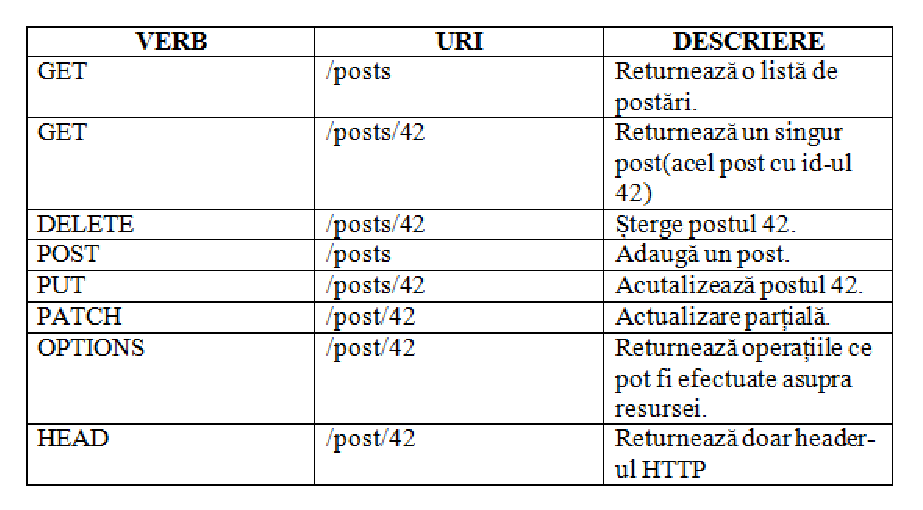
\includegraphics[width=12cm,height=9cm,keepaspectratio]{imagini/TabelVerbe.eps} %&
\paragraph{}
\textbf{Figura 4}
\end{center}


După cum se arată în \textbf{Figura 4}, folosind URI-ul și verbul corect, o resursă poate fi manipulată folosind operațiile CRUD (Create, Read, Update, Delete).
Atunci când se efectuează o cerere către server, serverul o analizează și construiește răspunsul pentru a returna datele sau rezultatul clientului. Fiecare răspuns este reprezentat de o stare și un status HTTP, ce ar trebui folosit pentru a informa clientul cu privire 
la rezultatul cererii.\cite{19}

Există cinci tipuri de statusuri HTTP:

\begin{itemize}
\item Informational (1xx)
\item Succes (2xx)
\item Redirection (3xx)
\item Client errors (4xx)
\item Server errors (5xx)
\end{itemize}

Fiecare tip de status are propriile detalii. De exemplu, în cazul în care cererea este efectuată cu succes, statusul răspunsului este ,,200 OK", după o cerere GET, dar este ,,201 CREATED" după o cerere POST. În cazul unui client care nu este autorizat să efectueze o cerere, statusul ,,403 Forbidden" ar trebui utilizat; dacă o resursă nu poate fi găsită, statusul ,,404 Not found" este utilizat.

\subsection{GET}
\paragraph{} GET este folosit pentru a citi o resursă. URI-ul specifică unde se găsește resursa pe care o citim, și se poate folosi header-ul Accept pentru a returna resursa într-un format specific. De exemplu cererea din \textbf{Figura 5} instruiește serverul să returneze conținutul în format JSON.


\vspace{1cm}

\begin{center}
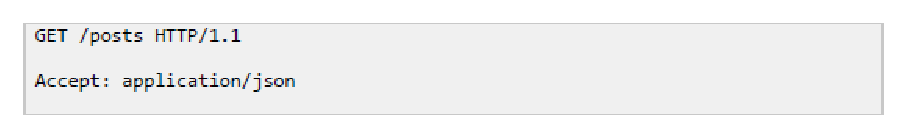
\includegraphics[width=12cm,height=9cm,keepaspectratio]{imagini/Get1.eps} %&
\paragraph{} \textbf{Figura 5}
\end{center}

\vspace{1cm}\newpage

Cererea din \textbf{Figura 6} instruiește serverul să returneze o resursă Post cu identificatorul 42, în format XML.

\begin{center}
\includegraphics[width=12cm,height=9cm,keepaspectratio]{imagini/Get2.eps} %&
\paragraph{}
\textbf{Figura 6}
\end{center}

\vspace{1cm}

O cerere GET este considerată una sigură, așadar aceasta nu ar trebui să modifice niciodată starea unei resurse.
Serverul răspunde de obicei unei cereri GET cu statusul \textbf{HTTP 200 OK} dacă totul decurge bine, \textbf{404 Not found} dacă URI-ul  pointează către o resură inexistentă, sau \textbf{400 Bad request} dacă cererea nu este corectă.\cite{19}

\subsection{POST}
\paragraph{} Când POST este folosit pentru a crea o resursă, datele resursei sunt trimise către server ca parte a corpului cererii. Serverul răspunde cu un status 201 CREATED dacă totul merge bine. Când este creată o nouă resursă, o bună practică este de a utiliza antetul Location în răspuns pentru a specifica URI-ul resursei nou create. Această bună practică aderă la principiul \textbf{HATEOAS}.\cite{19}

\paragraph{}
\textbf{Notă:} \emph{HATEOAS (Hypermedia as the Engine of Application State)
\paragraph{} Într-o aplicație REST, clientul trebuie să știe cât mai puține informații pentru a utiliza aplicația. În mod ideal, singurul lucru pe care clientul trebuie să îl știe este URI-ul punctului de intrare. Toate celelalte URI-uri trebuie să fie furnizate de către server folosind anteturile de localizare sau alte mecanisme (link-uri rel, de exemplu), pentru a informa clientul unde sunt restul resurselor. În acest fel clientul și serverul nu sunt legate și serverul ar putea schimba locația resursei fără a strica clientul. Acest principiu este baza  unui API REST bine conceput.
}

\subsection{PUT}
\paragraph{} PUT este folosit pentru a modifica o resursă. URI-ul specifică resursa care va fi modificată iar corpul cererii conține noile valori ale resursei. Răspunsul ar trebui să conțină statusul \textbf{200 OK} sau \textbf{204 No content} în cazul în care răspunsul nu conține resursa modificată. Nu este necesar să se returneze URI-ul resursei în antetul Location deoarece clientul știe deja acest URI. \cite{19}

PUT trebuie să fie \textit{idempotent}, ceea ce înseamnă că rezultatul unei cereri efectuate cu succes nu depinde de numărul de execuții a cererii. Trebuie să fie posibil să se efectueze două apeluri identice către server, iar serverul nu ar trebui să returneze erori; al doilea apel, pur și simplu actualizează resursa din nou, chiar dacă aceasta nu se schimbă.

\subsection{DELETE}
\paragraph{} DELETE este folosit pentru a șterge o resursă. Rezultatul poate fi \textbf{200 OK} sau \textbf{204 NO CONTENT} dacă răspunsul nu conține un body. Poate fi \textbf{404 Not found} dacă URI-ul nu este corect și resursa nu poate fi găsită.\cite{19}

\section{Proiect Web API}

\paragraph{} Template-ul  Web API este parte a template-ului de proiect ASP.NET MVC 5. Acesta este instalat implicit in Visual Studio 2012 și Visual Studio 2013. Pentru versiuni mai vechi de Visual Studio aceste template-uri trebuie instalate. Structura unei aplicații ASP.NET MVC 5 este prezentată în \textbf{Figura 7}.

\begin{center}
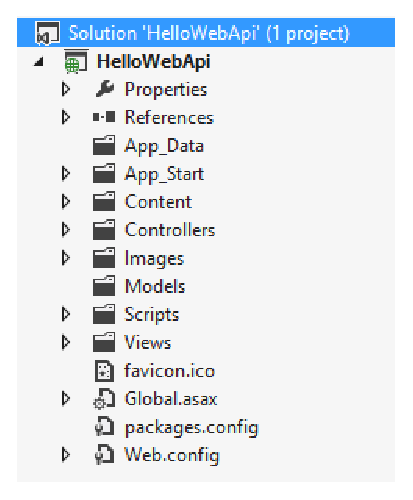
\includegraphics[width=12cm,height=9cm,keepaspectratio]{imagini/StructuraAPI.eps} 
\paragraph{}
\textbf{Figura 7}
\end{center}\newpage


Cele mai importante lucruri de evidențiat sunt:

\begin{itemize}
\item Directoarele \textbf{Controllers}, \textbf{Models} și \textbf{Views} sunt împrumutate din ASP.NET MVC. Web API folosește același șablon ca și MVC. Totuși, directorul \textbf{Views} nu este foarte folositor în contextul Web API, deși este posibil să se returneze un view către un client
\item Pe lângă directorul \textbf{Views}, mai sunt directoarele \textbf{Images}, \textbf{Scripts} și \textbf{Content}. Acestea nu sunt folosite de obicei, din moment ce un API este în general utilizat pentru a returna date, nu interfețe utilizator
\item Directorul \textbf{App\_Start} este folosit pentru a configura API-ul. Acesta conține diverse configurații pentru a seta comportamentul API-ului
\end{itemize}

Atunci când este creat, un proiect ASP.NET Web API conține un controller implicit(\textbf{Figura 8}).

\begin{center}
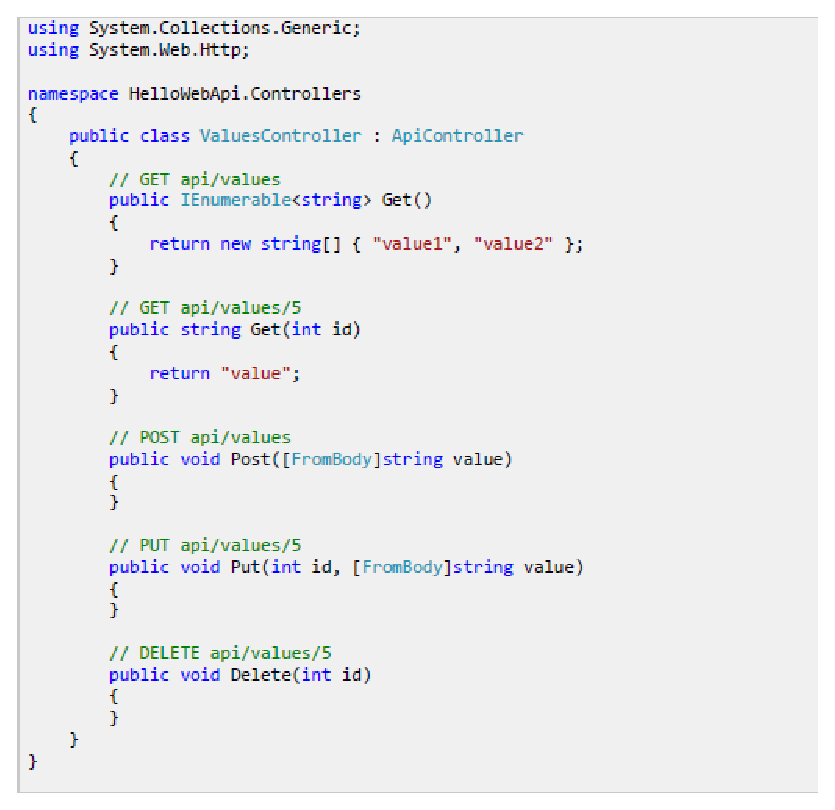
\includegraphics[width=12cm,height=9cm,keepaspectratio]{imagini/ControllerAPI.eps} 
\paragraph{}
\textbf{Figura 8}
\end{center}

\paragraph{} După cum se poate vedea în Figura 4, după instrucțiunile ,,using" și ,,namespace" se declară o nouă clasă, \textbf{ValuesController}. Această clasă moștenește din \textbf{ApiController}. Acest lucru este important deoarece, \textbf{ApiController} nu este ,,rudă" cu clasa de bază a controller-lor din ASP.NET MVC, chiar dacă au foarte multe similarități. Așadar \textbf{ApiController} deservește ca și clasă de bază pentru toate resursele ce vor fi expuse prin intermediul API-ului.

În interiorul clasei se pot observa toate verbele implicite utilizate în manipularea resurselor: \textbf{GET}, \textbf{POST}, \textbf{PUT}, \textbf{DELETE}. Numele metodelor din interiorul clasei este foarte important, din moment ce runtime-ul ASP.NET Web API folosește \textbf{convențiile} ca mecanism pentru a apela metoda corectă, pe care o cerere a formulat-o. Așadar cele două metode \textit{Get} sunt folosite pentru a returna o colecție de valori și pentru a returna o valoare cu un ID specific. Metodele \textit{Post} și \textit{Put} sunt folosite pentru a insera și modifica o resursă, în timp ce metoda \textit{Delete} este folosită pentru a șterge o resursă cu un id specific.

\paragraph{} Ca și o aplicație web ASP.NET MVC, proiectele Web API folosesc un sistem de rutare. Configurarea rutelor se efectuează într-un fișier denumit \textbf{WebApiConfig.cs}, în directorul \textbf{App\_Start}. \textbf{Figura 9} ilustrează conținutul acestui fișier.\cite{19}

\begin{center}
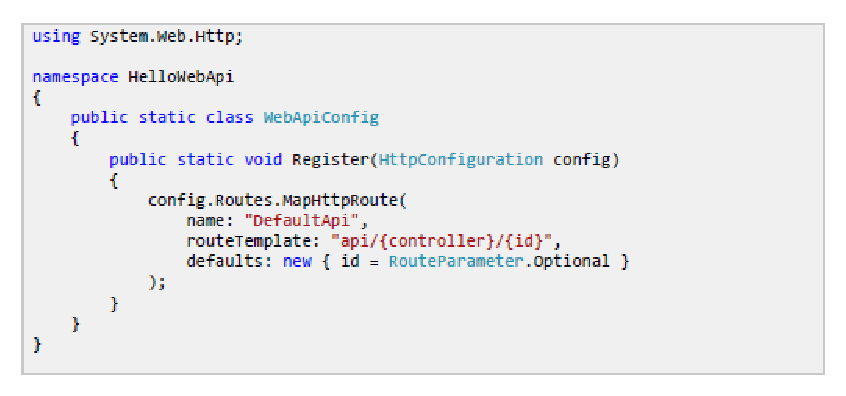
\includegraphics[width=12cm,height=9cm,keepaspectratio]{imagini/RutareAPI.eps} %&
\paragraph{}
\textbf{Figura 9}
\end{center}\newpage


\paragraph{} Această clasă conține o metodă ce este invocată din clasa \textbf{WebApiApplication}, din global.asax. Această metodă înregistrează rutele folosite de aplicație. Implicit, clasa ValuesController definită în \textbf{Figura 8}, răspunde la URI-ul \textit{/api/Values}. Este de evidențiat faptul că deși aceste rute sunt similare rutelor din ASP.NET MVC, sunt pe o stivă complet diferită. În cazul Web.API tipul rutei este \textbf{IHttpRoute} iar implementarea este conținută în assembly-ul \textbf{System.Web.Http}, care este un assembly complet nou, ce nu are nicio legătură cu \textbf{System.Web}. Fiecare rută are un nume și un template ce conține anumiți tokeni pentru a se potrivi cu șabloanele de intrare.\cite{19}


\section{Ciclul de viață al unei cereri}

\paragraph{} Atunci când un client trimite o cerere către o aplicație ASP.NET Web Api, cererea va trece prin trei straturi, pentru a fi procesată. Componentele principale ce au un rol activ în această procesare, sunt listate în \textbf{Figura 10}.

\begin{center}
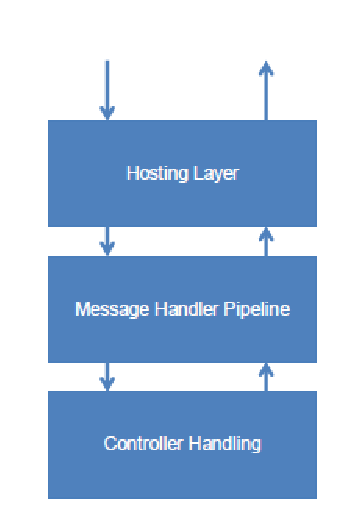
\includegraphics[width=12cm,height=9cm,keepaspectratio]{imagini/CicluCerere.eps} %&
\paragraph{}
\textbf{Figura 10}
\end{center}

Următorele straturi sunt folosite atunci când o cerere este procesată:
\begin{itemize}
\item Hosting Layer
\item Message Handler Pipeline
\item Controller Handling
\end{itemize}

\subsection{Hosting Layer}
\paragraph{} Primul strat este stratul de hosting, care primește cererea HTTP direct de la client. Stratul de hosting ar putea fi un server clasic de IIS(Internet Information Server) ce folosește mecanismul ASP.NET, sau o aplicație self-hosted.

Rolul stratului de hosting este de a primi cereri și de a le converti în instanțe de \textbf{HttpRequestMessage}, o clasă ce reprezintă cererea. Mesajul cererii este transmis mai jos către Message Handler Pipeline. Cum este contruită această cerere depinde de tipul de hosting.

\subsection{Message Handler Pipeline}
\paragraph{} Message Handler Pipeline reprezintă stratul de mijloc al arhitecturii prezentate. Acesta constă în înlanțuirea  de handlere ce pot fi folosite pentru a satisface nevoile aplicației. Fiecare handler este o instanță a clasei derivată din \textbf{HttpMessageHandler} ce are o metodă \textbf{SendAsync}, care primește o instanță a \textbf{HttpRequestMessage} și returnează un \textbf{HttpResponseMessage}.\cite{19}

Fiecare din aceste handlere are o referință către un InnerHandler, ce reprezintă următorul handler din secvență ce va fi apelat.
Cu această arhitectură, fiecare cerere poate fi pre-procesată sau post-procesată de multiple handlere ce fac diferite lucruri.

Exemple de handlere de mesaje sunt \textbf{HttpRoutingDispatcher} ce direcționează cererea pe baza unei rute și \textbf{HttpControllerDispatcher} ce trimite cererea către controller.
Aceste handlere sunt deja în secvență, de vreme ce sunt în colecția \textbf{HttpConfiguration.MessageHandlers}. Altele pot fi adăugate în colecție în timpul configurării aplicației Web API.

\subsection{Controller Handling}
\paragraph{} Acesta este ultimul strat. Stratul de controller handling primește mesajul cererii de la stratul anterior și apelează acțiunea controller-ului trimițând parametrii ceruți. Task-ul este îndeplinit de \textbf{HttpControllerDispatcher}, ultimul handler din secvență. Acesta, cu ajutorul \textbf{HttpControllerDescriptor}, obține o instanță a clasei ce implementează \textbf{IHttpInterface} și apelează metoda \textbf{ExecuteAsync} a acestei instanțe. Selectarea acțiunii corecte pentru a fi executată intră în îndatoririle metodei \textbf{ApiController.ExecuteAsync}, care bind-uiește parametrii, execută filtrele acțiunii (dacă sunt prezente), iar mai apoi execută acțiunea propriu-zisă.\cite{19}

Un \textbf{IActionResultConverter} convertește rezultatul acțiunii la o instanță \textbf{HttpResponseMessage}. Mesajul cererii este trimis către client folosind aceeași cale ca și a cererii.


\include{cap77}
\chapter{Arhitectura aplicației}
Aplicația este formată din trei module importante. 
Primul modul este reprezentat de aplicația client - aplicație Android, al doilea modul este reprezentat de server - aplicatie web și aplicația care se ocupă cu preluarea și prelucrarea datelor de pe Internet și depunerea acestora în baza de date aflată în cloud - aplicație Java Spring.
\section{Aplicația client}
Aplicația client este o aplicație pentru dispozitive mobile care au sistem de operare Android. Aceasta a fost implementată cu ajutorul limbajului Java utilizând ca și mediu de dezvoltare Android Studio, astfel că am folosit o serie de instrumente interactive care se îmbină în armonie pentru a crea o interfață prietenoasă, ușor de utilizat de către deținătorii de smartphone-uri Android. 
Aplicația a fost dezvoltată având ca și nivel API minim versiune 14, acoperind astfel 87,9\% din toate dispozitivele active în Google Play Store, începând cu versiunea de Android Ice Cream Sandwich. Am ales această versiune de API datorită faptului că permite utilizarea de funcționalități noi care în versiunire anterioare nu sunt disponibile, rezultând astfel un design mai modern și mai intuitiv. Mai mult, numărul de device-uri active cu un nivel API inferior este în scădere, de asemenea și numărul de aplicații dezvoltate pentru versiunile inferioare a scăzut semnificativ în ultima perioadă.
\section{Aplicația desktop Java}
Acest modul se ocupă cu preluarea și parsarea informatiilor despre produse cu ajutorul API-ului Jsoup HTML Parser\footnote{vezi capitolul 5 - Jsoup API}.\newpage Această aplicație se ocupă preluarea produselor de pe anumite site-uri și în funcție de fiecare categorie va rezulta o listă de produse care apoi va fi filtrată și în final alegându-se doar produsele pentru care se aplică reducere, pentru a nu stoca informații pe care nu le vom folosi ulterior. Atfel după preluarea datelor de pe Internet se asigură persistența acestora prin intermediul serviciului REST. 
\section{Aplicația server}
Aplicația server este reprezentată de un serviciu REST care a fost implementat cu ajutorul templatelul Web API regăsit în ASP.NET\footnote{vezi capitolul 6 - REST}
Acesta reprezintă legătura între cele două module prezentate anterior întrucât prin intermediul serviciului se depun datele în baza de date, se preiau datele din baza de date și se modifică cu ajutorul operațiilor REST. O interfață, ce definește contractul între server și viitorii clienți, conține toate metodele la care clienții vor avea acces. Aceste metode sunt implementate în clasa serviciului. 
Persistenta datelor este realizata într-o bază de date aflată în cloud\footnote{pentru detalii despre cloud computing vezi Capitolul 7 }. Comunicarea dintre baza de date și server este efectuată folosind ORM-ul (Object Relationing Model) Entity Framework. Acest model este util deoarece întreaga bază de date este cartografiată în server. Acest lucru înseamnă că pentru fiecare tabel din baza de date, este creată o clasă iar clasele vor fi puternic conectate intre ele. De asemenea orice modificare adusă bazei de date este ușor de integrat și în server.


\chapter{Capitolul 8}
\section{PromON}
%%poza siglaaa!!!
\textbf{Log In/Sign Up}
\paragraph{ }Meniul de start al aplicației client este reprezentat de fereastra de Log In/Sign Up care este afișată doar în cazul în care utilizatorul nu este deja autentificat. Aceasta cuprinde două text box-uri în care clientul își va introduce un e-mail și o parolă necesare pentru autentificare sau pentru crearea unui cont nou, caz în care va fi necesară o confirmare a parolei.

\begin{center}
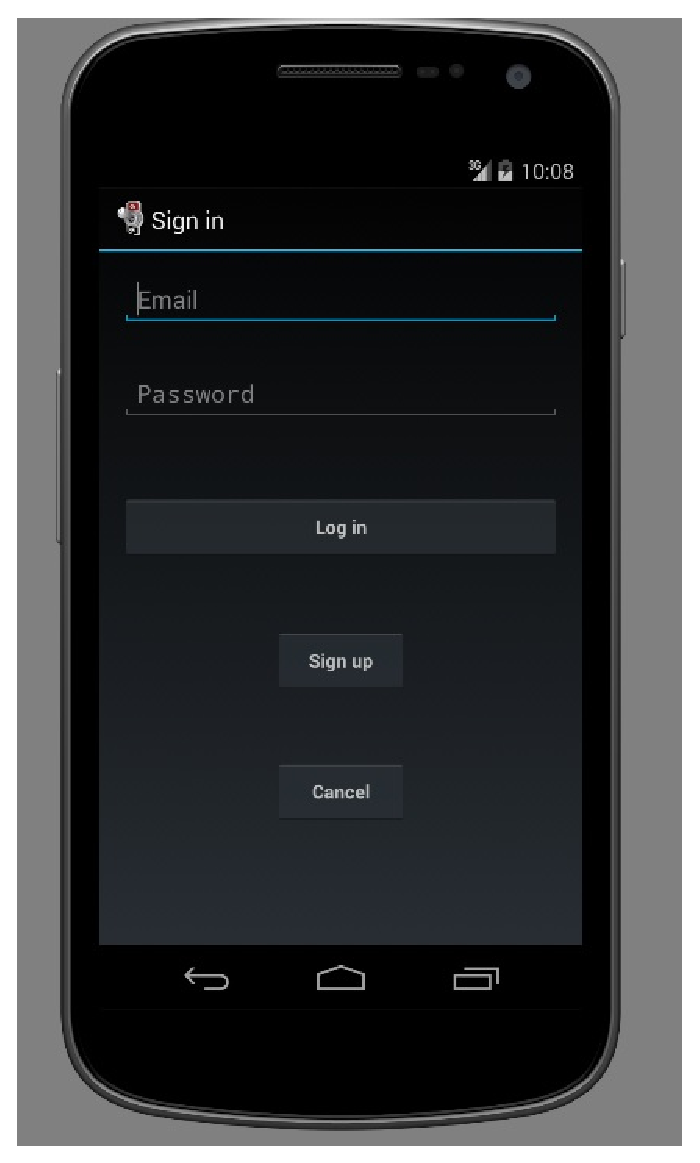
\includegraphics[width=12cm,height=9cm,keepaspectratio]{imagini/login.eps} %&
\paragraph{}
\textbf{Login}
\end{center}

\begin{center}
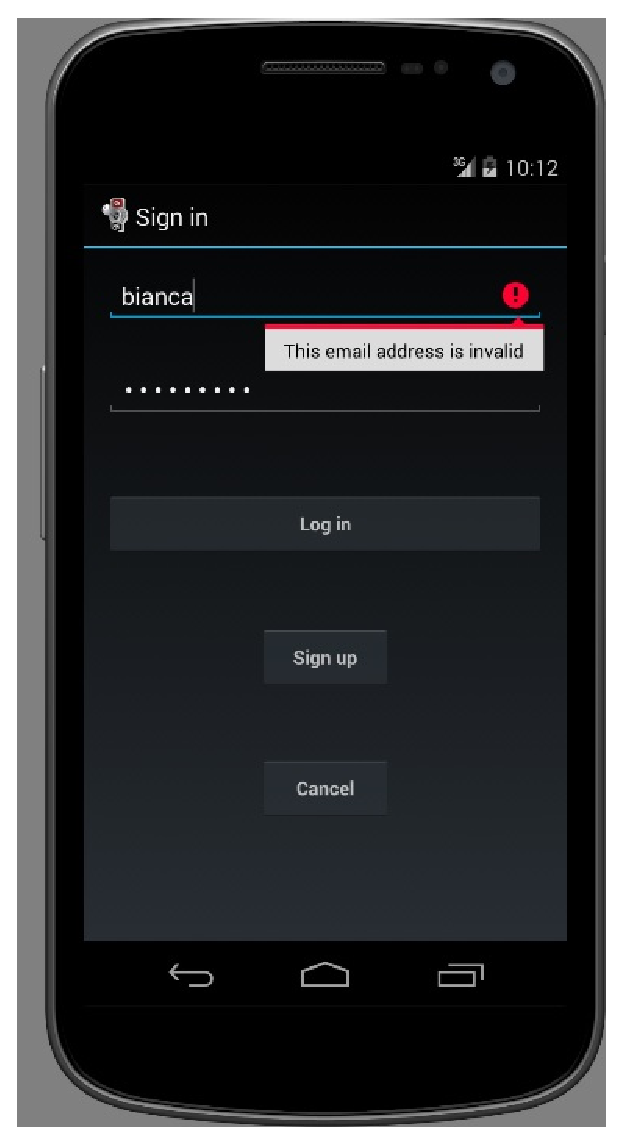
\includegraphics[width=12cm,height=9cm,keepaspectratio]{imagini/emailinvalid.eps} %&
\paragraph{}
\textbf{Atenționare e-mail invalid}
\end{center}

\begin{center}
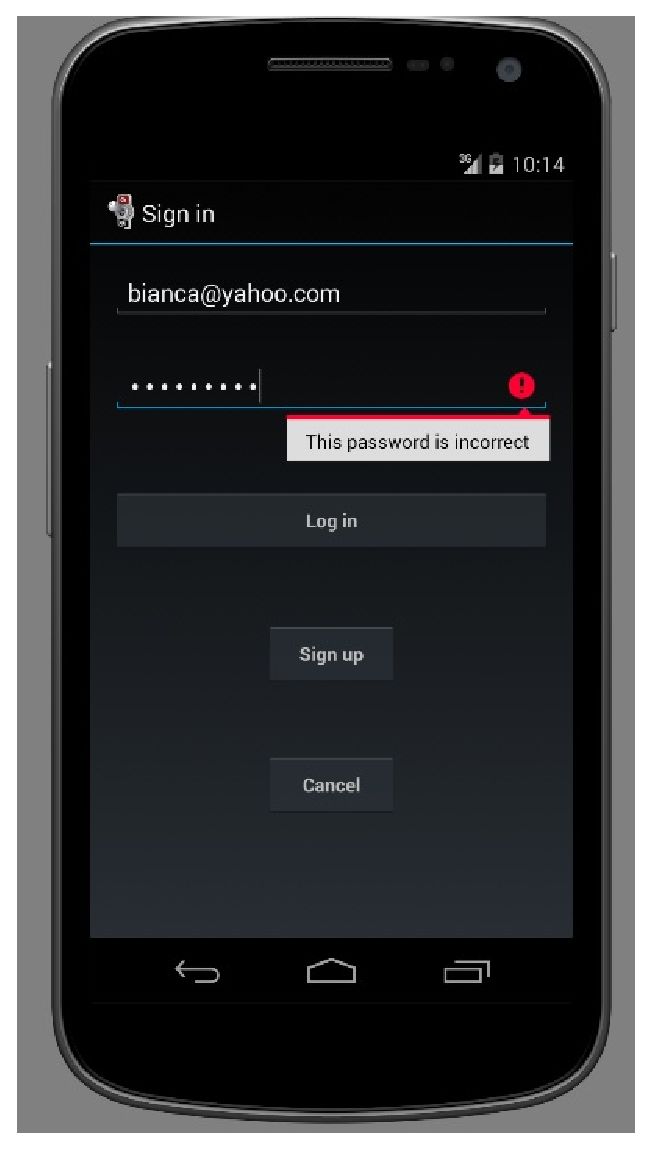
\includegraphics[width=12cm,height=9cm,keepaspectratio]{imagini/invalidpass.eps} %&
\paragraph{}
\textbf{Atenționare parolă invalidă}
\end{center}

\textbf{Pagina principală}
\paragraph{ }După conectare se va deschide o pagină în care, vor fi afișate primele 10 produse sortate în funcție de cel mai mare discount acordat. Acestea se vor schimba dupa 5 secunde timp în care dacă utilizatorul este interesat va putea apăsa pe butonul ,,cumpără'' care îl va redirecționa spre site-ul de unde poate achiziționa produsul.

\textbf{Meniul slide-in}
\paragraph{ }Pentru a oferi un design elegant și nu foarte încărcat, pentru a naviga prin celelalte funcționalități ale aplicației am ales să utilizez un meniu slider care va sta ascuns pe parcursul acțiunilor de pe o anumită pagină dar va putea fi oricând vizibil printr-o simplă atingere a ecranului dinspre stânga spre dreapta sau prin atingerea iconiței de meniu. Astfel toate modulele aplicației sunt grupate și pot fi accesate rapid și simplu, comunicarea între acestea fiind de asemenea printr-o simpla atingere a elementului din meniu corespunzător paginii care se dorește a fi deschisă.
Unul dintre motivele pentru care am ales să dezvolt aplicația pentru versiunile de Android pornind de la IceCreamSandwich este utilizarea acestui tip de meniu care din punctul meu de vedere are un impact mare fiind un instrument modern și din ce în ce mai utilizat în aplicații importante precum Facebook, YahooMail, GMail etc. Asfel, utilizatorii Android sunt obișnuiți cu utilizarea acestui navigator și pot folosi aplicația cu ușurință. 
%poza meniul meu si eventual poza meniu fb, mail?

\textbf{Categorii}
 \paragraph{ }Acest fragment al aplicației cuprinde o listă de categorii de produse disponibile, personalizate cu o iconiță sugestivă pentru impact vizual și un buton comutator prin care un client își poate alege metoda de afișare a categoriilor, sortate în funcție de nume, alfabetic, sau în functie de numărul de accesări, cele mai populare categorii fiind listate primele în acest caz.
\begin{center}
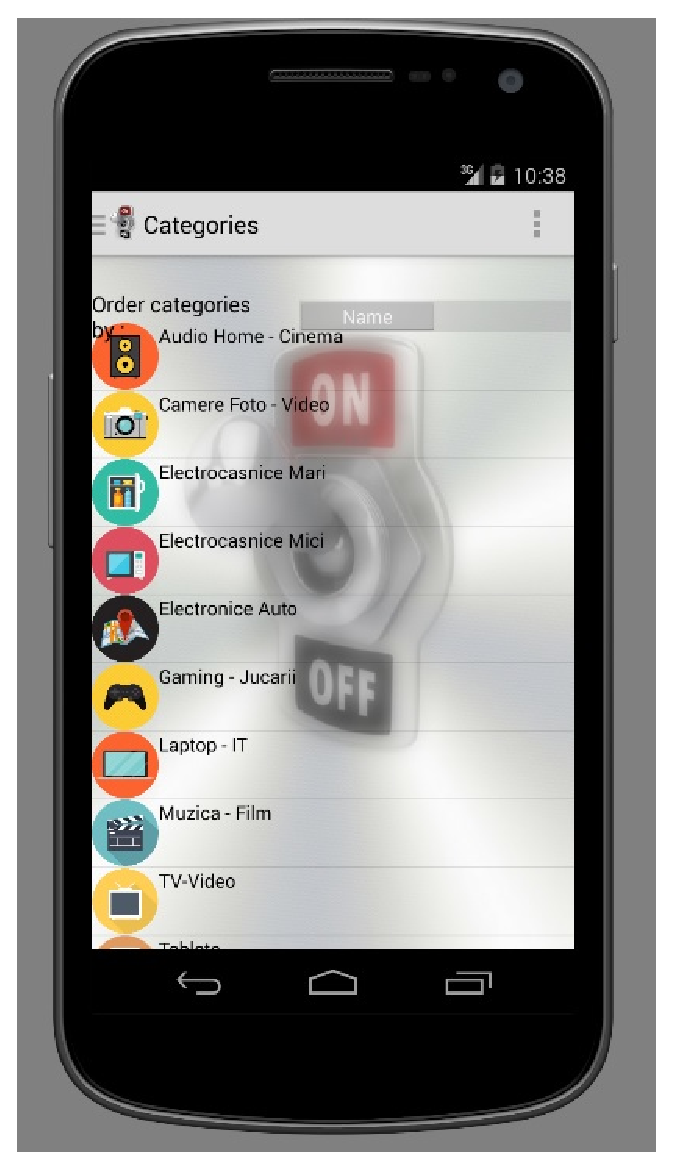
\includegraphics[width=12cm,height=9cm,keepaspectratio]{imagini/categorii.eps} %&
\paragraph{}
\textbf{Listă categorii sortate alfabetic}
\end{center}

\begin{center}
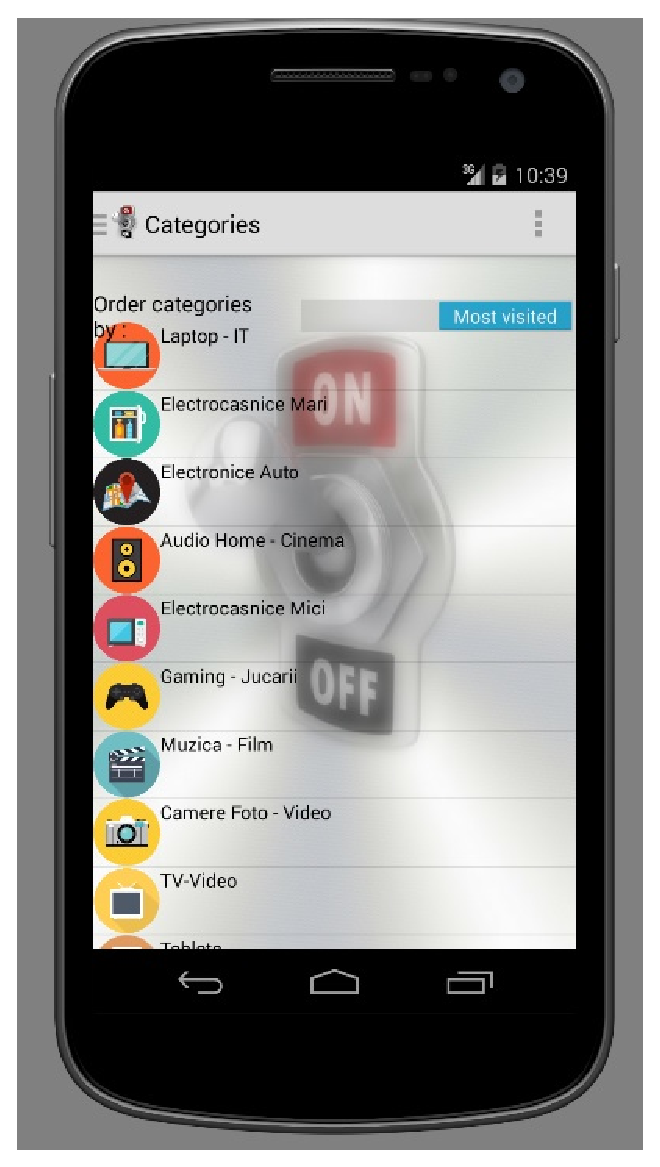
\includegraphics[width=12cm,height=9cm,keepaspectratio]{imagini/catgorii2.eps} %&
\paragraph{}
\textbf{Listă categorii sortate în funcție de numărul de accesări}
\end{center}

\textbf{Produse}
\paragraph{ }După ce utilizatorul selectează o categorie din listă, se deschide o nouă fereastră, ce cuprinde o listă cu produsele care apartin categoriei alese. De asemenea acestea pot fi sortate, utilizând un buton comutator, alfabetic sau descrescător după valoarea discountului care se oferă pentru fiecare produs în parte.
După ce alege produsul dorit, pentru a fi vizionat în detaliu se deschide o nouă fereastră în care se pot vizualiza prețul curent, prețul anterior, detalii despre produs și o poză semnificativă.  Această pagină corespunde cu pagina principală, în care sunt afișate însă doar 10 produse, considerate produsele de top. De asemenea, pentru a cumpăra un produs, apare un buton, care , o dată apăsat va deschide browserul principal al telefonului și va deschide pagina corespunzătoare produsului curent.

\textbf{Setări}
\paragraph{ } Meniul de setări cuprinde opțiunea de a alege o temă pentru aplicație prin selectarea acesteia dintr-un meniu drop-down. O dată selectată o temă, clientul trebuie să apese butonul Aplică pentru ca tema curentă să se modifice cu cea aleasă.  Acest fragment de aplicație este oferă posibilitatea utilizatorul de a-si personaliza aplicația, este util însă și pentru sănătatea ochilor întrucât în funcție de lumină este recomandat să alegem culori care să nu ne afecteze vederea. 

\begin{center}
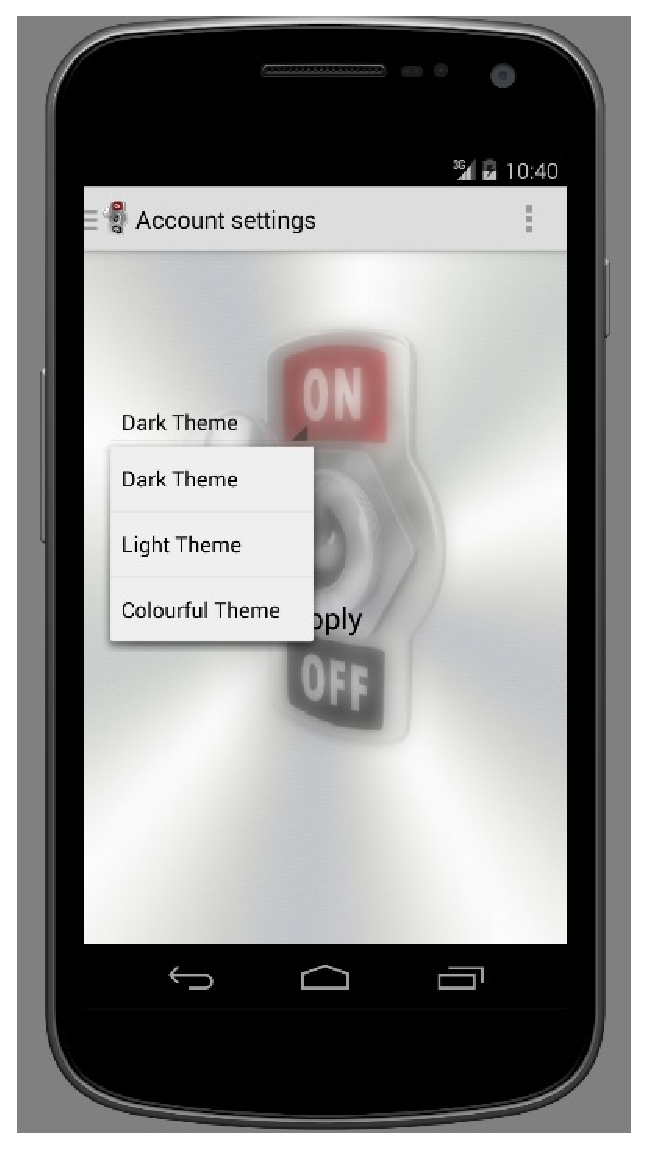
\includegraphics[width=12cm,height=9cm,keepaspectratio]{imagini/settings.eps} %&
\paragraph{}
\textbf{Pagină setări}
\end{center}

\textbf{Termeni și condiții}
\paragraph{ } Orice aplicație cuprinde o serie de termeni și condiții, aceștia au fost acceptați o dată cu instalarea aplicației, însă este de preferat să fie disponibili pentru o recitire ulterioară și în cazul în care utilizatorul nu este de acord să poată dezinstala aplicația.


\textbf{Log Out}
\paragraph{ } Acest fragment se referă la ieșirea din cont și o dată apăsat butonul de Log Out, utilizatorul va fi redirecționat către pagina de Log In, unde va putea să se autentifice cu un alt cont deja existent, să-și creeze un cont nou sau pur și simplu să iasă din aplicație.
\begin{center}
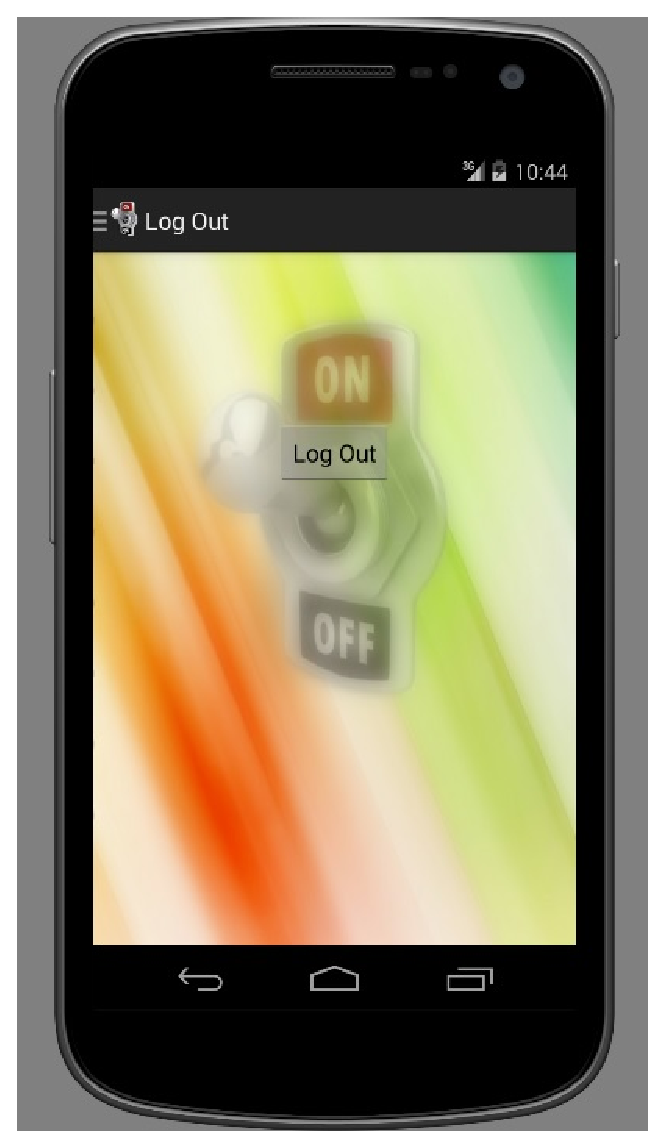
\includegraphics[width=12cm,height=9cm,keepaspectratio]{imagini/logout.eps} %&
\paragraph{}
\textbf{Pagină log out}
\end{center}


%%%%Find a product????



\begin{thebibliography}{99}

\addcontentsline{toc}{chapter}{\bibname}

\bibitem{1}
Onur Cinar, 2015, \emph{Android Quick APIs Reference}, Editura APRESS.

\bibitem{2}
Dave Smith, 2015, \emph{Android Recipes: A Problem-Solution Approach for Android 5.0},Editura APRESS.
\bibitem{3}
Wei-Meng Lee, 2012 \emph{BEGINNING Android 4 Application Development}, Editura Wrox Press

\bibitem{4}
Sayed Y. Hashimi and Satya Komatineni, 2009, \emph{Pro Android},
Editura APRESS.

\bibitem{5}
Open Handset Alliance, 2007, Industry Leaders Announce Open Platform for Mobile Devices. Press release., \newline\url{http://www.openhandsetalliance.com/press_110507.html}

\bibitem{6}
Google's Android parts ways with Java industry group,\url{ http://www.cnet.com/news/googles-android-parts-ways-with-java-industry-group/}

\bibitem{7}
General Android 2008,\newline\url{ http://code.google.com/android/kb/general.html}

\bibitem{8}
Native C application for Android, \newline\url{http://benno.id.au/blog/2007/11/13/android-native-apps}

\bibitem{9}
Android version history, \newline\url{http://en.wikipedia.org/wiki/Android_version_history#Pre-commercial_release_versions}

\bibitem{10}
http://www.oracle.com/technetwork/java/

\bibitem{11}
Barry Burd PhD, 2014, Beginning Programming with Java For Dummies, 4th Edition, Wiley eBooks

\bibitem{12}
Ştefan Tanasa, Cristian Olaru, Stefan Andrei, "Java de la 0 la expert", Polirom, 2003.

 \bibitem{13}
Yakov Fain, 2011, Java Programming 24-Hour Trainer, Wrox eBooks

 \bibitem{14}
Yvor Horton, 2011, Beginning Java , Java 7 Edition, John Wiley \& Sons, Inc.

\bibitem{15}
Adrian Deaconu, 2007, Programarea în C/C++ și aplicații , Grupul microInformatica, Cluj-Napoca

\bibitem{16}
Document Object Model (DOM). http://www.w3.org/: W3C., 2012

\bibitem{17}
Lawrence Rosen, OPEN SOURCE LICENSING, p.85 (Prentice Hall PTR, 1st ed. 2004)

\bibitem{18}
jsoup: Java HTML Parser, https://jsoup.org/

\bibitem{19}
Emanuele Delbono, 2013, ASP.NET Web API Succinctly, Syncfusion.

\bibitem{20}
Michael Collier, Robin Shahan, 2015, Fundamentals of Azure, Microsoft Press. Ed. APRESS.

\end{thebibliography}



\end{document}


